\pdfoutput=1
\pdfcompresslevel=9
\pdfinfo
{
    /Author Andrzej Fiedukowicz
    /Title Implementacja symulatora środowiska miejskiego na potrzeby systemu fuzji danych
    /Subject Symulacja środowiska miejskiego. Systemy Fuzji danych.
    /Keywords Symulacja, symulator, środowisko miejskie, fuzja danych, śledzenie obiektów, fuzja informacji
}
%\documentclass[a4paper,polish,onecolumn,oneside,floatssmall,11pt,titleauthor,wide,openright]{mwrep}
%\usepackage[scale={0.7,0.8},paper=a4paper,twoside]{geometry}
\documentclass[a4paper,onecolumn,oneside,12pt,wide,floatssmall]{mwrep}
% \usepackage{polish}
\usepackage{amsmath}
\usepackage{amsfonts}
\usepackage{amssymb}
\usepackage{amsthm}
\usepackage{bookman}

\usepackage{geometry}
\usepackage[utf8x]{inputenc}
\usepackage[T1]{fontenc}
% \usepackage{t1enc}
% \usepackage[pdftex, bookmarks]{hyperref}
\usepackage[pdftex, bookmarks=false]{hyperref}
\def\url#1{{ \tt #1}}

\usepackage{listings}

% marginesy
\textwidth\paperwidth
\advance\textwidth -55mm
%\linespread{2.0}
\oddsidemargin-0.9in
\advance\oddsidemargin 33mm
\evensidemargin-0.9in
\advance\evensidemargin 33mm
\topmargin -1in
\advance\topmargin 25mm
\setlength\textheight{48\baselineskip}
\addtolength\textheight{\topskip}
\marginparwidth15mm

\clubpenalty=10000 % to kara za sierotki
\widowpenalty=10000 % nie pozostawia wdów
\brokenpenalty=10000 % nie dzieli wyrazów pomiędzy stronami
\sloppy

\tolerance4500
\pretolerance250
\hfuzz=1.5pt
\hbadness1450

% ŻYWA PAGINA
\renewcommand{\chaptermark}[1]{\markboth{\scshape\small\bfseries \
#1}{\small\bfseries \ #1}}
\renewcommand{\sectionmark}[1]{\markboth{\scshape\small\bfseries\thesection.\
#1}{\small\bfseries\thesection.\ #1}}
\newcommand{\headrulewidth}{0.5pt}
\newcommand{\footrulewidth}{0.pt}
\pagestyle{uheadings}

\usepackage[pdftex]{color,graphicx}
\usepackage[polish]{babel}
\DeclareGraphicsExtensions{.png,.jpg}

% \textheight232mm
% \setlength{\textwidth}{\textwidth}
% \setlength{\oddsidemargin}{\evensidemargin}
% \setlength{\evensidemargin}{0.3cm}
\usepackage[sort, compress]{cite}

%\usepackage{multibib}
%\newcites{bk,st,doc,web}{Książki i~artykuły,Standardy i~zalecenia,Dokumentacja produktów,Publikacje i~serwisy internetowe}

\theoremstyle{definition}
\newtheorem{defn}{Definicja}[section]
\newtheorem{conj}{Teza}[section]
\newtheorem{conjmain}{Teza}
\newtheorem{exmp}{Przykład}[section]

\theoremstyle{plain}% default
\newtheorem{thm}{Twierdzenie}[section]
\newtheorem{lem}[thm]{Lemat}
\newtheorem{prop}[thm]{Hipoteza}
\newtheorem*{cor}{Wniosek}

\theoremstyle{remark}
\newtheorem*{rem}{Uwaga}
\newtheorem*{note}{Uwaga}
\newtheorem{case}{Przypadek}

\definecolor{ListingBackground}{rgb}{0.95,0.95,0.95}

\begin{document}

% kody źródłowe wplatane w tekst
\lstdefinestyle{incode}
{
basicstyle={\footnotesize},
keywordstyle={\bf\footnotesize\color{blue}},
commentstyle={\em\footnotesize\color{magenta}},
numbers=left,
stepnumber=5,
firstnumber=1,
numberfirstline=true,
numberblanklines=true,
numberstyle={\sf\tiny},
numbersep=10pt,
tabsize=2,
xleftmargin=17pt,
framexleftmargin=3pt,
framexbottommargin=2pt,
framextopmargin=2pt,
framexrightmargin=0pt,
showstringspaces=true,
backgroundcolor={\color{ListingBackground}},
extendedchars=true,
% title=\lstname,
captionpos=b,
% abovecaptionskip=1pt,
% belowcaptionskip=1pt,
frame=tb,
framerule=0pt,
}

% kody źródłowe z podpisem
\lstdefinestyle{outcode}
{
basicstyle={\footnotesize},
keywordstyle={\bf\footnotesize\color{blue}},
commentstyle={\em\footnotesize\color{magenta}},
numbers=left,
stepnumber=5,
firstnumber=1,
numberfirstline=true,
numberblanklines=true,
numberstyle={\sf\tiny},
numbersep=10pt,
tabsize=2,
xleftmargin=17pt,
framexleftmargin=3pt,
framexbottommargin=2pt,
framextopmargin=2pt,
framexrightmargin=0pt,
showstringspaces=true,
backgroundcolor={\color{ListingBackground}},
extendedchars=true,
% title=\lstname,
captionpos=b,
% abovecaptionskip=1pt,
% belowcaptionskip=1pt,
frame=tb,
framerule=0.1pt,
}

\renewcommand*\lstlistingname{Wydruk}
\renewcommand*\lstlistlistingname{Spis wydruków}

\pagenumbering{roman}
\renewcommand{\baselinestretch}{1.0}
\raggedbottom

\begin{titlepage}
    % Strona tytułowa
    \vbox to\textheight{\hyphenpenalty=10000
    \begin{center}
	\begin{tabular}{p{107mm} p{9cm}}
	    \begin{minipage}{9cm}
	      \begin{center}
	      Politechnika Warszawska \\
	      Wydział Elektroniki i~Technik Informacyjnych \\
	      Instytut Informatyki
	      \end{center}
	    \end{minipage}
	    &
	    \begin{minipage}{8cm}
	    \begin{flushleft}
	     \footnotesize
	      Rok akademicki 2012/2013
	    \vspace*{2.75\baselineskip}
	    \end{flushleft}
	    \end{minipage} \\
	\end{tabular}
	\vspace*{3.75\baselineskip}
	\par\vspace{\smallskipamount}
	\vspace*{2\baselineskip}{\LARGE Praca dyplomowa inżynierska\par}
	\vspace{3\baselineskip}{\LARGE\strut Andrzej Fiedukowicz\par}
	\vspace*{2\baselineskip}{\huge\bfseries Implementacja symulatora ruchu obiektów w środowisku miejskim na potrzeby systemu fuzji danych
	\par}

	\vspace*{7\baselineskip}
	\hfill\mbox{}\par\vspace*{\baselineskip}\noindent
	\begin{tabular}[b]{@{}p{3cm}@{\ }l@{}}
	    {\large\hfill } & {\large }
	\end{tabular}
	\hfill
	\begin{tabular}[b]{@{}l@{}}
	Opiekun pracy: \\[\smallskipamount]
	{\large dr inż. Rafał Biedrzycki}
	\end{tabular}\par
	\vspace*{4\baselineskip}
    \begin{tabular}{p{\textwidth}}
    \begin{flushleft}
	\begin{minipage}{7cm}
	Ocena \dotfill
	\par\vspace{1.6\baselineskip}
	\dotfill
	\par\noindent
	\centerline{\footnotesize Podpis Przewodniczącego} \par
	\centerline{\footnotesize Komisji Egzaminu Dyplomowego}\par
	\end{minipage}
    \end{flushleft}
    \end{tabular}
    \end{center}}

    % Życiorys
    \newpage\thispagestyle{empty}
    \begin{tabular}{p{5cm} p{12cm}}
    \begin{minipage}{5cm}
    \center
    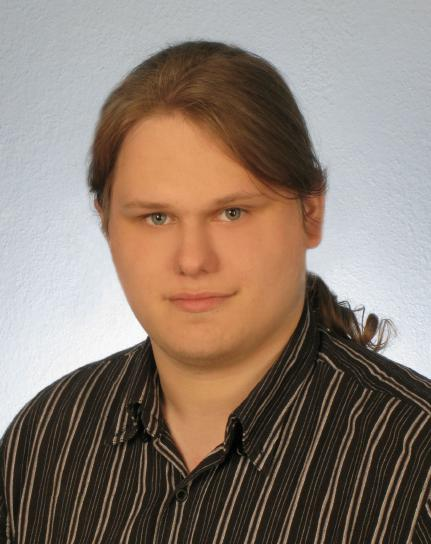
\includegraphics[height=5.8cm,width=4.5cm]{img/foto.jpg}
    \end{minipage}
    &
    \begin{minipage}{12cm}
    \begin{flushleft}
    \par\noindent\vspace{1\baselineskip}
    \begin{tabular}[h]{l l}
    {\normalsize\it Specjalność:} & Informatyka -- \\
    & Inżynieria systemów \\
    & informatycznych \\
    \end{tabular}
    \par\noindent\vspace{1\baselineskip}
    \begin{tabular}[h]{l l}
    {\normalsize\it Data urodzenia:} & {\normalsize 2 maja 1990~r.}
    \end{tabular}
    \par\noindent\vspace{1\baselineskip}
    \begin{tabular}[h]{l l}
    {\normalsize\it Data rozpoczęcia studiów:} & {\normalsize 22 luty 2010 r.}
    \end{tabular}
    \par\noindent\vspace{1\baselineskip}
    \end{flushleft}
    \end{minipage}
    \end{tabular}
    \vspace*{1\baselineskip}
    \begin{center}
	{\large\bfseries Życiorys}\par\bigskip
    \end{center}

    \indent
    Nazywam się Andrzej Fiedukowicz, urodziłem się 2 maja 1990 roku w Warszawie. W roku 2003 ukończyłem Szkołę Podstawową w Chocianowie, a w roku 2006 Gimnazjum nr 1 w Józefowie. Naukę kontynuowałem w IV Liceum Ogólnokształcącego im. Adama Mickiewicza w Warszawie, które ukończyłem zdając maturę w 2009 roku. W lutym roku 2010 rozpocząłem studia na wydziale Elektroniki i Technik Informacyjnych Politechniki Warszawskiej na kierunku Informatyka w toku studiów wybierając specjalizację Inżynieria Systemów Informatycznych. Od maja 2012 roku pracuję zawodowo jako programista języka C++.
    \par
    \vspace{2\baselineskip}
    \hfill\parbox{15em}{{\small\dotfill}\\[-.3ex]
    \centerline{\footnotesize podpis studenta}}\par
    \vspace{3\baselineskip}
    \begin{center}
 	{\large\bfseries Egzamin dyplomowy} \par\bigskip\bigskip
    \end{center}
    \par\noindent\vspace{1.5\baselineskip}
    Złożył egzamin dyplomowy w dn. \dotfill
    \par\noindent\vspace{1.5\baselineskip}
    Z wynikiem \dotfill
    \par\noindent\vspace{1.5\baselineskip}
    Ogólny wynik studiów \dotfill
    \par\noindent\vspace{1.5\baselineskip}
    Dodatkowe wnioski i uwagi Komisji \dotfill
    \par\noindent\vspace{1.5\baselineskip}
    \dotfill

    % Streszczenie
    \newpage\thispagestyle{empty}
    \vspace*{2\baselineskip}
    \begin{center}
	{\large\bfseries Streszczenie}\par\bigskip
    \end{center}

    {\itshape
    \par{
    Praca opisuje podejście do tworzenie symulatorów mających stanowić źródło danych dla systemów fuzji danych oraz wprowadza do związanej z tym problamatyki.
	}    
    \par{
	W pracy opisano również proces tworzenia modelu ruchu obiektów w środowisku miejskim. Stworzono model uwzględniający specyfikę systemów fuzji danych. Zaprezentowano podejście do tworzenia ogólnej architekutry aplikacji wykorzystującej zaproponowany model oraz wykorzystano tę architekturę by stworzyć konkretną implementację systemu symulującego zdolnego do współpracy z systemem fuzji daych.
	}
	\par{
	W ramach pracy przeprowadzono także badania wydajnościowe, które pozwoliły okreslic jakiego rodzaju ograniczenia programowo-sprzętowe są kluczowe z punktu widzenia możliwości omawianych systemów.
	}
    }
    \vspace*{1\baselineskip}

    \noindent{\bf Słowa kluczowe}: {\itshape symulator, środowiso miejskie, fuzja danych.}
    \par
    \vspace{4\baselineskip}
    \begin{center}
	{\large\bfseries Abstract}\par\bigskip
    \end{center}
    \noindent{\bf Title}: {\itshape Implementation of urban environment simulator for purposes of data fusion system.
    }\par
    \vspace*{1\baselineskip}
    {\itshape
    \par{
    This thesis describes approach to creating simulator feeding data fusion systems and introduces to problems associated with it.
	}
    \par{
    This thessis also describes process of creating movement model of objects in urban environment designed to work as part of data fusion system. Model that meets data fusion specific requirements was created. Aproach to creating general architecture of application using created model was shown together with its specific implementation capable of working with data fusion system.
	}
	\par{
	This thessis was also a base to conduct some performance benchmarks which allowed to determine which kind of software or hardware limitation is currently crucial from the described systems point of view.
	}
    }
    \vspace*{1\baselineskip}

    \noindent{\bf Key words}: {\itshape simulation, urban environment, data fusion}

\end{titlepage}

% ex: set tabstop=4 shiftwidth=4 softtabstop=4 noexpandtab fileformat=unix filetype=tex spelllang=pl,en spell:


\tableofcontents
% \addcontentsline{toc}{chapter}{{Przedmowa1}{vii}}{vii}

% \chapter*{Spis tablic, rysunków i~wydruków}
% \listoftables
% \listoffigures
% \lstlistoflistings

%\setlength{\baselineskip}{7mm}
\newpage
\pagenumbering{arabic}
\setcounter{page}{1}

\chapter{Wprowadzenie}

\par{
Systemy, które pozwalają na zbieranie informacji z wielu źródeł i ich łączenie w celu uzyskania spójnego obrazu obserwowanych zjawisk nazywane są systemami fuzji danych \cite{jdl}. Tego rodzaju systemy zdają się być kluczowym elementem rozwoju współczesnej informatyki, ponieważ coraz częściej mamy do czynienia z sytuacjami, w których dane rozproszone są dookoła globu, a dopiero zebranie i przeanalizowanie ich całości pozwala zaobserwować pewne zjawiska i wyciągnąć odpowiednie wnioski.
\par{
Tego rodzaju badania wymagają odpowiedniego wsparcia ze strony symulacji komputerowej. Dla ich prowadzenia zdaje się być bowiem kluczowe stworzenie systemów mogących symulować dane o charakterystyce bliskiej danym rzeczywistym, a jednocześnie pozwalające odtworzyć je w formie nie zaszumionej, by porównać wyniki systemu fuzji z rzeczywistym obrazem symulowanego świata.
}
\par{
Niniejsza praca opisuje sposób podejścia do projektowania tego rodzaju symulatora. Implementowany system jest symulatorem środowiska miejskiego z systemem miejskiego monitoringu – tego rodzaju system zdaje się doskonale pasować do specyfiki systemów rozproszonych, ze względu na różnorodność zbieranych odczytów, problemy związane z synchronizacją czasu i wieloma źródłami danych, przez które należy w tym wypadku rozumieć czujniki systemu monitoringu.
}
\section{Cel pracy}
\par{
Celem pracy jest zaprojektowanie architektury i zaimplementowanie symulatora środowiska miejskiego. W ramach realizacji tego celu należy stworzyć odpowiedni model środowiska miejskiego.
}
\par{
Projektowany symulator powinien stanowić źródło danych testowych dla systemu ich fuzji. Szczegółowe wymagania dla referencyjnej implementacji opisano w rozdziale 3.1.
}
\chapter{Podstawy teoretyczne}
\section[Symulacja komputerowa][Symulacja komputerowa]{Symulacja Komputerowa}

\subsection{Wstęp}
\par{
Ludzkość od zarania dziejów stara się analizować otaczający ją świat. Nie bez powodu. Zrozumienie zasad, według których funkcjonuje otaczająca nas rzeczywistość zdaje się znacząco ułatwiać naszą egzystencję co w prostej linii prowadzi do tego, że samo dążenie do zgłębienia prawideł świata da się wytłumaczyć odwołując się bezpośrednio do ewolucji --- osobniki lepiej rozumiejące otaczający świat potrafią lepiej się mierzyć z pojawiającymi się w nim przeciwnościami.
}

\par{
Zasadniczo ludzkie badania działają na dwóch płaszczyznach --- dążą do przewidywania przyszłości i pozwalają podejmować coraz lepsze reakcje na bieżące zdarzenia.
}

\par{
Przez wiele lat ludzie prowadzili rozliczne badania starające się wyjaśniać naturę świata --- z początku nieco chaotycznie (co nie znaczy, że bez znaczących sukcesów) --- u zarania nauki w starożytnej Grecji, gdy cała nauka zamknięta była w jedną dziedzinę nazywaną ogólnym mianem Filozofii.
Wraz z rozwojem ludzkości nasze podejście do nauki jako takiej ewoluowało. I tak już w XVII wieku Kartezjusz wysuwał postulaty, że podstawą nauki powinny być pewne abstrakcyjne narzędzia jak matematyka i logika na bazie których buduje się teorię innych dziedzin. Współcześnie niewiele odsunęliśmy się od myśli Kartezjusza --- podstawą naszych badań zdaje się być matematyka, na którą nakładane są inne dziedziny jak fizyka i chemia, których wypadkową są nauki przyrodnicze.
}

\par{
Warto zwrócić uwagę, że nasza nauka układa się w sposób warstwowy --- kolejne warstwy pozwalają nam odcinać się od reguł obowiązujących w małej skali i budować teorie dla skali większej. Jest to szczególnie uzasadnione w świetle odkryć XX wieku, jak ogólna teoria względności.
}

\par{
Oczywiście nadal wiele naukowych tez ma charakter czysto empiryczny i często jest to wystarczające dla określonych zastosowań --- w końcu po dziś dzień nauka służy ludziom a nie odwrotnie.
}

\par{
Mamy więc do czynienia z pozornym rozłamem nauki --- z jednej strony formalizmy pozwalające na precyzyjny, spójny i co najważniejsze --- jednoznaczny, opis określonych zjawisk. Z drugiej strony badania empiryczne, na podstawie których często wyszukuje się potencjalnych dróg rozwoju w sposób analityczny. Obie te metody uzupełniają się wzajemnie --- niektórych badań praktycznych nie sposób zaplanować bez określonych reguł i znajomości niektórych torii a jednocześnie niektóre teorie (w zasadzie większość) nie powstały by gdyby nie konkretne obserwacje rzeczywistości.
}

\par{
Symulacja komputerowa jest narzędziem badań empirycznych, choć ściśle wykorzystuje specyficzny aparat matematyczny. Stosując ją wykorzystujemy bowiem teorie w pewnej skali, by odtworzyć zachowania i obserwować ich skutki w innej (zwykle większej), np. symulując ruch cząsteczek cieczy według określonych fizyką zasad by obserwować zachowanie cieczy jako całości w określonych warunkach.
}

\par{
Czym jest więc symulacja komputerowa? Symulacja to proces, który pozwala przy użyciu reguł jednej skali obserwować zjawiska w innej. Słowo komputerowa odnosi się do konkretnej realizacji --- z wykorzystaniem maszyn cyfrowych. Dobrym podsumowaniem ukazującym funkcję symulacji komputerowej zdaje się być schemat przedstawiający trzy filary współczesnej nauki wg. prof. Michała Kleibera \cite{Kleiber} widoczny na rysunku \ref{filaryNauki}
\begin{figure}[htb]
    \begin{center}
	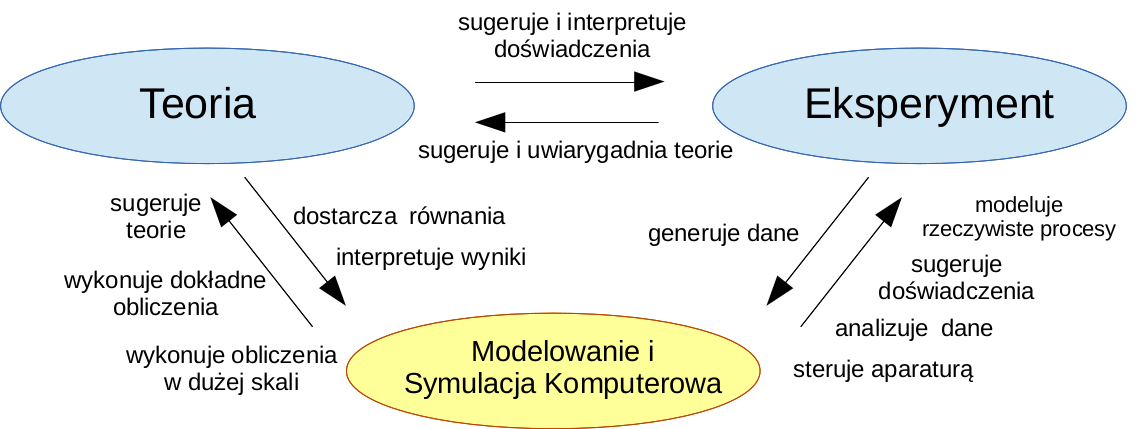
\includegraphics[angle=0,scale=0.4]{img/triada_poznania.png}
	\caption{Trzy filary poznawcze współczesnej nauki.}
	\label{filaryNauki}
    \end{center}
\end{figure}
}

\subsection{Filozofia symulacji komputerowej}

\subsubsection{Postulat Laplace'a}
\par{
W roku 1814 Pierre Simon Laplace opublikował artykuł pod tytułem: \textit{Filozoficzny esej na temat prawdopodobieństwa} (fran. \textit{Essai philosophique sur les probabilites}) \cite{Laplace}, w którym wysunął następujący postulat:
}
\par{
\textit{Umysł, który by znał siły działające w danej chwili w przyrodzie oraz wzajemne położenie wszystkich istotności, z których ona się składa, gdyby zdołał ująć je i poddać analizie --- w jednym wzorze zawarłby ruchy największych ciał niebieskich i najdrobniejszych atomów. Nie byłoby dla niego nic niepewnego i zarówno przyszłość, jak i przeszłość świata byłyby obecne dla jego oka ...
}}
\par{
\textit{... Jesteśmy tak dalecy od chwili, kiedy poznamy wszystkie siły przyrody i różne formy ich oddziaływania, że nie byłoby godnym filozofa negowanie pewnych zjawisk jedynie dlatego, że nie można ich objaśnić przy obecnym stanie wiedzy. Jesteśmy zobowiązani do badania zjawisk tym dokładniej, im trudniej przychodzi nam uznać je za istniejące.}
}

\par{
Współczesna nauka odsunęła się nieco od tej koncepcji. Po pierwsze przyjmuje się (mając na względzie zasady fizyki kwantowej), że świat nie opiera się o deterministyczne zasady --- co w zasadzie obala postulat Laplace'a. Po drugie natomiast, zgodnie z zasadą nieoznaczoności Heisenberga \cite{Heisenberg} nie jest możliwe uzyskanie pełnego obrazu świata ponieważ każda jego obserwacja wpływa na jego stan --- co uniemożliwia wykorzystanie postulatu Laplace'a w praktyce.
}
\par{
Obalenie teorii Laplace'a nie oznacza bynajmniej, że nie pozostaje ona poza światem nauki --- nadal ma ona bardzo duże znaczenie filozoficzne oraz nadal aktualna pozostaje jej druga część. Ponadto, w wielu sytuacjach zakłada się, że zasada ta nadal obowiązuje --- jednym z takich miejsc jest symulacja komputerowa.
}
\par{
Podstawą w zasadzie każdej symulacji komputerowej jest stan symulowanych obiektów oraz oddziaływania między nimi. Zakłada się, że symulator zna \textbf{wszystkie} zasady obowiązujące w symulowanym świecie jak i stan wszystkich obiektów w nim występujących i w związku z tym jest w stanie określić przyszłość symulowanego układu --- jest to stan, o którym wspominał Laplace'a, a symulator można by w tym kontekście potraktować jako demona Laplace'a. Warto zwrócić uwagę, że w podejściu takim nie ma nic zdrożnego, ani sprzecznego ze współczesną nauką --- przede wszystkim dlatego, że ograniczenie symulacji do ciągu przyczyn i skutków nie obniża zwykle jej wartości w kwestii celu jaki się przed nią stawia.
}

\subsubsection{Precyzja komputerów}
\par{
Kolejnym problem w pewien sposób uniemożliwiający przyrównanie rzeczywistości do symulacji komputerowej jest fakt, że współczesne komputery przechowują dane w sposób skwantowany (binarny). W związku z tym nie sposób opisać na nim danych o charakterze ciągłym z dowolną precyzją.
}
\par{
Choć zdawać by się mogło, że w świetle współczesnych badań, ograniczenie to przestaje mieć sens, ponieważ przyjmuje się, że wszelkie zjawiska w przyrodzie mają charakter kwantowy, to należy wziąć pod uwagę jak małe są kwanty o których mówi ta teoria.
}
\par{
Długość Plancka (czyli minimalna obserwowalna we wszechświecie odległość) wynosi 
\begin{center}
$l_P = c \ t_P = \sqrt{\frac{\hbar G}{c^3}} = 1,616 199(97) \times 10^{-35} m$
\end{center}
co oznacza, że aby zapisać na komputerze dokładne położenie obiektu w trójwymiarowej kostce o boku długości jednego metra potrzebowali byśmy ok. $3.5 \times 10^{65}$ terabajta pamięci. Przy obecnej technologii zdaje się więc, że dokładność komputera jest zasadniczym problemem uniemożliwiającym dokładne odwzorowanie rzeczywistości.
}

\subsubsection{Praktyczne znaczenie ograniczeń}
\par{
W praktyce, wyżej wymienione ograniczenia nie są zwykle krytyczne. Zazwyczaj bowiem symulacja ma za zadanie upraszczać wygląd rzeczywistości, a więc nadmierna precyzja jest w wręcz niewskazana.
}
\par{
Warto jednak zdawać sobie sprawę, że symulacja komputerowa jest jedynie pewnym przybliżeniem rzeczywistości i z samej swojej natury obarczona jest zasadniczym błędem --- i właśnie znalezienie takiego sposobu symulacji by błąd w możliwie małym stopniu wpływał na aspekty istotne z punktu widzenia celu symulacji zdaje się być istotą jej projektowania.
}

\subsection{Zastosowanie symulacji}

\subsubsection{Przewidywanie zdarzeń}
\par{
Podstawowym zdaniem stawianym przed symulacjami komputerowymi zdaje się być przewidywanie różnego rodzaju zdarzeń. Znając zasady według których funkcjonują pewne zjawiska, jesteśmy w stanie do pewnego stopnia określić jak będą rozwijały się te zjawiska w przyszłości.
}
\par{
Niektóre z tych zjawisk potrafiliśmy przewidywać już przed erą symulacji komputerowej --- albo przy użyciu klasycznego aparatu matematycznego albo przy użyciu własnej intuicji i doświadczenia. Jednak symulowanie zjawisk w celu przewidywania ich rozwoju przenosi przewidywanie przyszłości na zupełnie nowy poziom.
}
\par{
Na symulację możemy wpływać --- tj. sprawdzać jak będzie reagowała na poszczególne bodźce ze świata zewnętrznego. Możemy także sterować jej przebiegiem --- tj. w miejscach gdzie pojawia się niepewność związana z metodyką symulacji wybrać konkretny wariant rozwiązania problemu.
Dzięki temu, jesteśmy w stanie, w krótkim czasie wytworzyć i przeanalizować wiele scenariuszy wydarzeń i na podstawie tych doświadczeń podejmować działania (w szczególności realne działania prewencyjne).
}
\par{
Przykładem tego rodzaju zastosowań jest symulowanie przebiegu huraganu, pozwalające przewidywać jego rozwój, kierunek i szybkość przemieszczania się w zależności od licznych, często samych w sobie trudnych do przewidzenia okoliczności. Na podstawie tego rodzaju symulacji uruchamia się służby kryzysowe w odpowiednich rejonach, informuje się mieszkańców o zagrożeniu, czy zarządza ewakuację.
}

\subsubsection{Badania i eksperymenty}
\par{
Drugi typ zastosowań ma ścisły związek z badaniami naukowymi.
Opisując model pewnych zjawisk, przy użyciu symulatora jesteśmy w stanie sprawdzać reakcję całego układu na naszą ingerencję jak i obserwować jego zachowanie w stanie zamkniętym. Tego rodzaju badanie może często uzmysławiać pewne zjawiska w innej skali, niż ta na której rozpatrywany jest układ w modelu symulacji.
}
\par{
Przeprowadzanie niektórych eksperymentów w świecie realnym jest często problematyczne, kosztowne lub wręcz niemożliwe. Symulowanie eksperymentów zdaje się pozwalać w znacznym stopniu usprawniać badania, a także wskazywać kierunki dalszego rozwoju. Jednocześnie najbardziej udane eksperymenty często powtarza się w rzeczywistości by uzyskać bardziej precyzyjny i pewny obraz.
}
\par{
Przykładem zastosowania w tym sektorze może być np. wspominana już symulacja zbiornika z wodą na poziomie pojedynczych cząsteczek by symulować jej zachowanie w konkretnych sytuacjach (np. uderzenie). Mając do dyspozycji taki symulator możemy zaobserwować jak reaguje tafla wody na uderzenie i np. wysnuć teorię na temat związku długości fali na wodzie z siłą uderzenia.
}

\subsubsection{Testowanie}
\par{
Często spotykanym problemem, na który napotykają inżynierowie jest niemożność testowania ich rozwiązań w realnych warunkach. W takich sytuacjach z pomocą często przychodzą komputerowe symulacje. Dostarczają one danych do badań, lub pozwalają obserwować reakcje układu na działanie wdrażanego systemu.
}
\par{
Symulator opisywany w niniejszej pracy został stworzony z myślą o właśnie takim zastosowaniu. Ma on za zadanie generować dane wyjściowe dotyczące ruchu w środowisku miejskim przeznaczone jako wejście dla systemu śledzenia obiektów, który przystosowany został do pracy z realnymi danymi.
}
\par{
Rozwiązanie wykorzystujące symulator jest tańsze, szybsze oraz znacznie prostsze i może w znacznym stopniu wyprzedzać bieżące czasy.
Zebranie realnych danych na temat pojazdów poruszających się po mieście jest zadaniem nie łatwym. Kamery z funkcją rozpoznawania obiektów są dopiero raczkującą technologią a ich umieszczenie w całym mieście jest bardzo kosztowne. Uzyskanie realnych danych potrzebnych do testowania skuteczności systemu śledzenia zdaje się więc być praktycznie niemożliwe.
}
\par{
Z pomocą przychodzą symulatory --- za ich pomocą możemy wytworzyć takie dane, jakich powinna nam dostarczyć hipotetyczna kamera. Nałożyć na nie odpowiednie szumy i zapisać razem z o wiele szerszymi danymi realnymi pozwalającymi analizować skuteczność wykorzystanych rozwiązań.
}
\par{
Dzięki temu, praca nad systemami śledzenia może postępować niezależnie od prac nad systemami monitoringu. Takie podejście sprawia że w sytuacji stworzenia i wdrożenia odpowiedniej realnej bazy sprzętowej będzie istniało już gotowe oprogramowanie mogące w pełni wykorzystać jej możliwości.
}
\par{
Wykorzystanie symulatorów do testowania zdaje się pozwalać na oszczędzanie dużej ilości zasobów i może prowadzić do skrócenia czasu badań pozwalając na unikanie kłopotliwych przygotowań do realnego testowania w trakcie koncepcyjnego opracowywania projektowanego systemu.
}

\subsubsection{Wizualizacja (także interaktywna)}
\par{
Ostatnim, acz nie najmniej istotnym z zastosowań symulatorów jest tworzenie wizualizacji w tym wizualizacji interaktywnych.
}
\par{
Organoleptyczne przekazywanie informacji jest bardzo istotne z punktu widzenia funkcjonowania człowieka --- dane dostarczone w sposób nieprzetworzony są zwykle niezrozumiałe lub wymagają dużych nakładów czasu by wyciągnąć z nich potrzebne informację. Ponieważ często symulator ma za zadanie zaprezentować ogólny pogląd na symulowane zjawisko, typowo wraz z symulatorem dostarczany jest system pozwalający zwizualizować jego pracę.
}
\par{
Praktyczne zastosowanie tego rodzaju tandemu zdaje się być bardzo szerokie. Pozwala to na prezentowanie sedna złożonych zjawisk, ułatwia przekazywania informacji, pozwala na obserwowanie zjawisk, do których odruchowej analizy człowiek jest całe życie przyzwyczajany. Dzięki temu często w sposób heurystyczny jesteśmy w stanie wyznaczyć pewne prawidłowości, których zasadność często sprawdzana jest dokładnie albo analitycznie albo z wykorzystaniem tego samego symulatora i dołączonego do niego modułu analizującego dane.
}
\par{
Prezentując dane przy użyciu odpowiedniej wizualizacji, jesteśmy w stanie przekazać złożone informacje w sposób intuicyjnie zrozumiały. Jest to cenna właściwość szczególnie dla edukacji czy wszelkiego rodzaju ciał doradczych współpracujących z podmiotami nie operującymi naukową nomenklaturą.
}
\par{
Powołując się ponownie na przykład symulacji cząstek wody by obserwować ich powierzchnię, wynikiem takiego symulatora było by zapewne położenie poszczególnych cząstek wody. Jednak chcąc widzieć realną powierzchnię --- często z uzyskanych danych wytworzymy trójwymiarowy obraz dający nam wrażenie jakbyśmy pracowali z realną cieczą.
}
\par{
Wizualizowanie wszelkich zjawisk zdaje się być nierozłącznie związane z ich symulowaniem i stanowi istotny element a w wielu sytuacjach cel egzystencji symulatorów jako takich.
}

\subsection{Model symulacji komputerowej}
\subsubsection{Definicja modelu}
Modelem w symulacji komputerowej nazywamy zasady, wedle których funkcjonuje symulacja, uwzględniający wszelkie zmienne wejściowe i wyprowadzający z nich zmienne wyjściowe z uwzględnieniem upływu czasu.
\par{
W literaturze \cite{PodstawyModelowania} można spotkać następującą, nieco bardziej ścisłą definicję:
Model \textit{to operator przekształcający zadane zmienne wejściowe X(t) w zmienne wyjściowe Y(t) czyli 
\begin{center}
$Y(t) = H_{t} \times X(t).$
\end{center}
}
}.

\subsubsection{Oczekiwane cechy modelu}
\par{
Przed modelami do symulacji najczęściej stawiane są trzy wymagania \cite{KotowskiTronczyk,WykladyJanczewski}:
\begin{enumerate}
\item Wymaganie jednoznaczności --- oznacza to, że operator modelu jest zależnością funkcyjną, tzn. że jeden zbiór danych wejściowych daje dokładnie jedną odpowiedź.
\item Wymaganie spójności (rozwiązywalności) --- oznacza to, że elementy modelu nie przeczą sobie nawzajem (są matematycznie spójne).
\item Wymaganie stabilności --- wymaganie to, oznacza, że niewielkie zmiany danych wejściowych nie powinny pociągać za sobą gwałtownych zmian w danych wyjściowych.
\end{enumerate}
}

\par{
Należy jednak zwrócić uwagę, iż niekiedy symulowany system posiada właściwości przeczące tej zasadzie --- nietrudno wyobrazić sobie na przykład symulację nacisku na jakiś obiekt, który po przekroczeniu pewnej krytycznej wartości siły nacisku łamie się, powodując diametralną zmianę wyglądu całego systemu (w wyniku reakcji łańcuchowej). 
}

\subsection{Taksonomia modeli}
\par{
Literatura [KotowskiTronczyk,PodstawyModelowania,WykladyJanczewski] podaje wiele kryteriów podziału modeli, poniżej zestawiono najbardziej ostre spośród nich.
}

\subsubsection{Podział ze względu na istnienie czasu}
\par{
\begin{itemize}
\item model dynamiczny --- znacznie bardziej popularny, upływ czasu jest uwzględniany w modelu i ma wpływ na wartości zmiennych wyjściowych.
\item model statyczny --- nie uwzględnia upływu czasu lub wartości zmiennych wyjściowych nie zależą od niego w żaden sposób.
\end{itemize}
}

\subsubsection{Podział ze względu na model czasu}
\par{
Dotyczy tylko modeli dynamicznych.
\begin{itemize}
\item model ciągły w czasie --- istnieje możliwość wyznaczenia wartości parametrów wyjściowych dla dowolnej chwili czasowej.
\item model dyskretny w czasie --- istnieje możliwość wyznaczenia wartości parametrów końcowych tylko dla przeliczalnego zbioru chwil czasowych.
\end{itemize}
}

\subsubsection{Podział ze względu na determinizm}
\par{
\begin{itemize}
\item model deterministyczny --- dla danego stanu początkowego daje zawsze taki sam wynik.
\item model niedeterministyczny --- wynik działania modelu nie jest zdeterminowany w momencie zadania stanu wejściowego.
\end{itemize}
}
\par{
Warto mieć na względzie, że modele niedeterministyczne niejako stoją w sprzeczności z postulatem Laplace'a jak i z postawionym wyżej wymaganiem jednoznaczności. Należy jednak pamiętać, że w typowym przypadku narzędziem programistycznym dla symulacji operującej na modelu niedeterministycznym będzie symulator liczb pseudolosowych, który choć wykazuje cechy probabilistyczne charakterystyczne dla liczb losowych, w rzeczywistości bazuje na deterministycznych zdarzeniach --- w praktyce więc każda komputerowa implementacja symulatora będzie miała charakter deterministyczny.
}

\subsubsection{Podział ze względu na oddziaływanie ze światem zewnętrznym}
\par{
\begin{itemize}
\item model autonomiczny --- tworzy zamknięty układ i nie uwzględnia żadnych możliwości interakcji z jego zewnętrzem.
\item model nieautonomiczny --- pozwala na dostarczanie bodźców (pobudzeń, wartości) z zewnątrz, które mają wpływ na zmienne wyjściowe.
\end{itemize}
}

\subsubsection{Podział ze względu na rodzaj związków między wejściem a wyjściem}
\par{
\begin{itemize}
\item model liniowy --- zmienne wyjściowe są związane ze zmiennymi wejściowymi przy użyciu liniowych funkcji.
\item model nieliniowy --- wykorzystuje funkcje nieliniowe do obliczania wartości parametrów wyjściowych.
\end{itemize}
}

\subsubsection{Podział ze względu na sposób tworzenia}
\par{
\begin{itemize}
\item model dedukcyjny --- reguły modelu pochodzą na podstawie teorii opisującej modelowane zjawisko.
\item model empiryczny --- reguły są tworzone na podstawie obserwacji zachowań modelowanego zjawiska, tak by model miał podobne obserwowalne właściwości.
\end{itemize}
}

\subsection{Modelowanie}
\par{
Proces tworzenia modeli pewnych zjawisk (np. na potrzeby symulacji komputerowej) nazywany jest modelowaniem. Proces ten, stanowi często wyzwanie dla przystępujących do niego inżynierów ze względu na bardzo wysoką złożoność zagadnień jak i konieczność dobierania miejsc, które model będzie upraszczał względem rzeczywistości, tak by zachować zasadność tworzenia modelu.
}

\subsubsection{Aspekty tworzenie modeli}
\par{
Przystępując do modelowania jakichkolwiek zjawisk poprawnym podejściem jest zwrócenie uwagi na następujące aspekty \cite{KotowskiTronczyk}:
\begin{itemize}
\item \textbf{cel} --- celowi tworzenia modelu powinny być podporządkowane wszystkie związane z nim działania. Należy pamiętać, że to model istnieje dla celu a nie odwrotnie. Cel symulacji stanowi punkt odniesienia, do którego należy często powracać i podporządkowywać mu decyzje podejmowane podczas modelowania.
\item \textbf{poziom uproszczenia} --- model z samej swojej natury musi być pewnym uproszczonym odpowiednikiem wycinka rzeczywistości. Jego stopień skomplikowania nie może być zbyt wysoki, przez wzgląd na ograniczenia dostępnych metod jego praktycznej implementacji. Z drugiej strony wybranie modelu nadmiernie uproszczonego może prowadzić do zagubienia pewnych specyficznych zachowań symulowanego zjawiska --- co może fałszować obraz symulacji. Dobrym określeniem porządanego stopnia uproszczenia modelu mogą być słowa Alberta Einsteina \cite{Wplyw}: \textit{Wszystko powinno zostać uproszczone tak bardzo, jak to tylko możliwe, ale nie bardziej.}
\item \textbf{potrzeby eksperymentu} --- niezwykle często zdarza się, że zjawisko modelowane jest z zamiarem przeprowadzenia ściśle określonego eksperymentu. Mając taką świadomość, jesteśmy w stanie łatwiej dobrać możliwe uproszczenia, a co ważniejsze pozbyć się wielu niepotrzebnych zależności z proponowanego modelu.
\item \textbf{poprawność} --- model uznaje się za poprawny, jeśli poddany każdemu możliwemu wejściu zachowa się wystarczająco podobnie do realnego zjawiska poddanego bodźcom odpowiadającym temu wejściu. Określenie, czy dane wyjście jest wystarczająco podobne do wyjścia realnego jest decyzją jaką podejmuje modelujący, mając na względnie różne aspekty modelu a w szczególności cel jego tworzenia.
\item \textbf{przydatność} --- model uznawany jest za przydatny gdy jego złożoność rośnie wolniej niż wykładniczo względem ilości zmiennych wykorzystywanych do jego opisu \cite{KotowskiTronczyk}. Modele zagadnień o złożoności wykładniczej mogą być poprawne, jednak ich precyzyjny opis jest często nieprzydatny i wymagane jest ich uproszczenie, by rozwiązywać symulowane zagadnienie z mniejszą dokładnością (np. heurystycznie) ale ciągle wystarczająco dobrze z punktu widzenia symulacji, a jednocześnie w realnie dostępnym czasie.
\item \textbf{wiarygodność} --- wiarygodność modelu określa na ile użytkownik jest przekonany o jego poprawności, szczególnie bazując na obserwacji wyników jego działania i organoleptycznym porównaniu tych wyników z realnym zjawiskiem. Wiarygodność modelu jest szczególnie istotna w przypadku symulacji przeznaczonych do wizualizacji określonych zjawisk.
\end{itemize}
}

\subsubsection{Zasadność modelu}
\par{
Model jako taki musi posiadać pewne cechy by był przydatny do jakichkolwiek zastosowań. Zastosowanie wyżej sformułowanych kryteriów doboru, powinno zapewnić, że model będzie właściwie sformułowany, jednak warto mieć dodatkowo na względzie  aspekty, wedle których można ocenić zasadność istnienia zaproponowanego przez nas modelu \cite{WykladyJanczewski}.
\begin{itemize}
\renewcommand{\labelitemi}{$\bullet$}
\item Badanie modelu nie powinno być bardziej złożone od badanie właściwego zjawiska.
\item Model powinien zachowywać się w sposób zbliżony do modelowanego zjawiska (zwłaszcza w kwestiach związanych ze swoim celem).
\end{itemize}
}


\section[Fizyczne modele dynamiki Newtona][Fizyczne modele dynamiki Newtona]{Fizyczne modele dynamiki Newtona}

\par{
Do stworzenia odpowiedniego modelu symulacji komputerowej, oprócz znajomości metodyki modelowania, wymagana jest znajomość teorii stojącej za modelowanym zjawiskiem oraz aparatu matematycznego dla niej odpowiedniego. Nie wydaje się jednak koniecznym by w ramach pracy tego rodzaju przybliżać podstawy fizyki klasycznej w postaci zasad dynamiki Newtona stanowiących w dzisiejszym świecie wiedzę powszechną.
}
\par{
Jednakże, zasady dynamiki Newtona operują na dwóch podstawowych modelach reprezentacji obiektów, z pośród których dla celów symulacji należy wybrać jeden mając świadomość związanych z tym konsekwencji. W związku z tym podstawowe cechy tych modeli zostaną omówione w tej pracy.
}

\subsection{Dynamika bryły sztywnej}
\par{
Model bryły sztywnej uwzględnia kształt i wymiary obiektu poruszającego się w przestrzeni. Jego podstawą jest założenie, że każdy obiekt ma strukturę jednostajnej, sztywnej (niezmieniającej kształtu pod względem czynników zewnętrznych) oraz nie absorbującej energii bryły, która poddawana jest wszelakim oddziaływaniom.
}
\par{
W związku z tym, że model bryły sztywnej zakłada wymiarowość obiektów, posiadają one w tym modelu sześć stopni swobody, które określają ich położenie w trójwymiarowej przestrzeni:
\begin{itemize}
\item trzy związane z ruchem postępowym
\renewcommand{\labelitemi}{$\bullet$}
	\begin{itemize}
	\item szerokość (położenie na osi X)
	\item wysokość (położenie na osi Y)
	\item głębokość (położenie na osi Z)
	\end{itemize}
\item trzy związane z ruchem obrotowym
	\begin{itemize}
	\item kąt \textit{roll} (obrót wokół osi X)
	\item kąt \textit{yaw} (obrót wokół osi Y)
	\item kąt \textit{pitch} (obrót wokół osi Z)
	\end{itemize}
\end{itemize}
Wymienione stopnie swobody zobrazowano na rysunku \ref{ryp}
\begin{figure}[htb]
    \begin{center}
	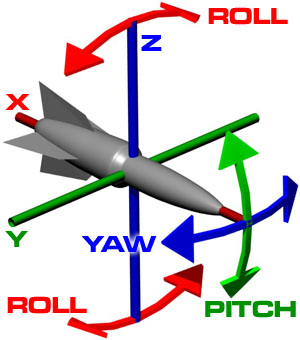
\includegraphics[]{img/xyz_ryp.jpg}
	\caption{Stopnie swobody bryły sztywnej \cite{Bryla}}
	\label{ryp}
    \end{center}
\end{figure}
}
\par{
Podstawową cechą jaką rzuca się w oczy przy opisywaniu tego modelu jest fakt, że opisuje on nie tylko pozycję ale i obrót obiektu (uwzględniając jego bryłę). Jest to więc model pozwalający na bezpośredni przekład wartości modelu fizycznego na obserwowalne przy użyciu zmysłów właściwości. Konsekwencją tego jest także możliwość naturalnego z punktu widzenia modelu fizycznego symulowania zderzeń niesprężystych. Ewentualne zderzenia sprężyste muszą być rozpatrywane poza  modelem fizycznym.
}
\par{
Jednocześnie wymaganie jednolitości całej bryły w tym modelu sprawia, że jej częściowa parametryzacja (np. wydzielenie oddzielnych właściwości szyby samochodu od jego karoserii) może być utrudniona i będzie musiała być najprawdopodobniej dokonana poza samym modelem fizycznym.
}
\par{
Podstawową wadą tego modelu jest dość wysoki stopnień złożoności ze względu na konieczność przejścia w wielu obliczeniach z rachunku skalarnego na rachunek wektorowy (zamiast pędu moment pędu itd.). Nie jest to stopnień złożoności, który mógłby stanowić wyzwanie dla współczesnej bazy sprzętowej, jednakże skomplikowanie obliczeń oznacza również zwiększenie kosztów (w szczególności czasowych) wytwarzania oprogramowania. Jest to argument, który należy brać pod uwagę bilansując koszta względem korzyści odnoszonych w wyniku zastosowania bardziej złożonych i precyzyjnych modeli.
}

\subsection{Dynamika punktu materialnego}
\par{
Model punktu materialnego nie uwzględnia kształtu i fizycznego charakteru poruszającego się w przestrzeni ciała. W tym modelu przyjmuje się, że ciało (a więc cała masa) skupione jest w przestrzeni o zerowych wymiarach (punkcie). Tego rodzaju uproszczenie znacząco obniża skomplikowania rachunków związanych z ruchem ciał, jednak uniemożliwia rozpatrywanie ich ruchu obrotowego jak i nie jest w stanie bez dodatkowego wsparcia zapewnić spójnego opisu zderzeń obiektów (dwa punkty nie mogą się zderzyć gdyż nie mają wymiarów).
}

\par{
Ponieważ punkt materialny nie ma wymiarów, posiada zaledwie trzy stopnie swobody, związane z położeniem, nie jest natomiast opisywany przez obroty (jak bryła sztywna):
\begin{itemize}
\item szerokość (położenie na osi X),
\item wysokość (położenie na osi Y),
\item głębokość (położenie na osi Z).
\end{itemize}
}

\par{
Jak wspomniano podstawową korzyścią płynącą z zastosowania takiego modelu zdaje się być uproszczenie obliczeń a więc zmniejszenie kosztów implementacji.
}
\par{
Do wad tego rozwiązania należy zaliczyć fakt, że wiele aspektów dotyczących obiektów w środowisku --- w tym bardzo podstawowych, jak obroty --- będą musiał być rozpatrywane odrębnie od modelu fizycznego. Większa ilość odrębnych od siebie modeli prowadzi w typowym wypadku do pewnych anomalii dających wrażenie nierealistycznego działania systemu.
}
\par{
Choć powyższe porównanie wyraźnie wskazuje, że zastosowanie modelu bryły sztywnej pozwala na bardziej spójne i co za tym idzie bardziej realistyczne przedstawienie rzeczywistości. Należy jednak mieć na względzie, że realne decyzje projektowe tego typu uwzględniają bilans zysku i kosztu a nie tylko zyski. W związku z tym, wybranie jednego z tych dwóch modeli jest istotnym wyzwaniem projektowym.
}

\section[Systemy fuzji danych][Systemy fuzji danych]{Systemy fuzji danych}
\par{
\textit{Fuzją danych} nazywa się \textit{proces łączący dane w celu oczyszczenia estymaty i predykcji stanu} \cite{revisionsJDL}, co jest uogólnieniem wcześniejszej definicji \cite{jdl} mówiącej, że \textit{Fuzja danych to proces obsługujący asocjację, korelację i wiązanie ze sobą danych i informacji z jednego lub wielu źródeł w celu uzyskania lepszej pozycji i tożsamości obiektu oraz możliwie trafnej i precyzyjnej ocenie sytuacji i zagrożenia.}
}
\par{
Obie powyższe definicje zdają się oddawać kwintesencję fuzji danych, którą jest zbieranie wielu danych o niedużej wartości jednostkowej w celu uzyskania szerokiego obrazu o dużej wartości końcowej.
}

\subsection{Rodzaje fuzji}
\par{
Systemy fuzji danych dzieli się ze względu na charakter danych poddawanych obróbce. Fuzją \textbf{danych} nazywa się procesy wykorzystujące dane pozbawione wstępnej obróbki lub ograniczające wstępną obróbkę do wyrównania dziedzin danych pochodzących z różnych źródeł. Systemy fuzji danych operują na danych nieprzetworzonych, np. właściwościach fizycznych sygnałów analogowych.
}
\par{
Bardziej rozpowszechniona od fuzji danych jest fuzja \textbf{informacji} nazywana również fuzją \textbf{cech} lub fuzją \textbf{właściwości} --- operująca na danych obrobionych, mających znaczenie na wyższym poziomie abstrakcji. Przykładem tego rodzaju systemu może być system operujący na danych dostarczanych z inteligentnych kamer w środowisku miejskim --- analizujący konkretne informacje o znanym charakterze (np. położenie obiektu) w celu uzyskania szerszych informacji na jego temat (np. śledzenie jego pozycji w czasie).
}
\par{
Rzadziej spotykanymi ale także wymienianymi w literaturze \cite{sroka08} są systemy fuzji \textbf{decyzji}. O tym przypadku mówi się, kiedy przetwarzanie danych przed samą fuzją idzie jeszcze o krok dalej --- tzn. na podstawie danych przed fuzją wypracowywana jest pewna decyzja. W takim przypadku dopiero niezależne decyzje z wielu źródeł są łączone w celu wypracowania rozwiązania ogólnego. Oznacza to, że daną w takim rozumieniu jest jakaś zmienna o charakterze sterującym sama sobie będąca wnioskiem z dostarczonych informacji, natomiast zadaniem systemu fuzji jest wybranie sumarycznej decyzji systemu nie wnikając w wewnętrzne funkcjonowanie poszczególnych swoich części a jedynie w poddecyzje.
}
\par{
Da się wyraźnie dostrzec, że poszczególne typy fuzji różnią się stopniem obróbki danych przed wejściem do systemu. W związku z tym systemy fuzji danych wydają się być bardziej złożone ale jednocześnie tracące najmniejszą ilość informacji. Zastosowane konkretnego rodzaju fuzji zależy ściśle od dziedziny zastosowania i intencji twórcy systemu --- nie sposób jest poszeregować wyników poszczególnych typów systemów w kategorii lepszy-gorszy.
}
\subsection{Model JDL}
\par{
Lata doświadczeń nad systemami fuzji danych pozwoliły na wypracowanie pewnych wzorców ich funkcjonowania stanowiących swoiste ramy dla wszystkich nowych systemów. Ilość modeli powstałych w czasie badań jest zauważalnie duża, jednak większość z nich zdaje się być jedynie szczególnym przypadkiem modelu zwanego modelem JDL.
}
\par{
Model ten ma pochodzenie militarno-wojskowe. Został on opracowany przez \textit{Data Fusion Subpanel of the Joint Directors of Laboratories} (JDL) w 1985 roku \cite{jdl}. W związku z tym nomenklatura używana do jego opisu jak i cele jakie stawia się przed tym modelem są ściśle związane z potrzebami wojskowymi. Nic jednak nie stało na przeszkodzie żeby wykorzystać tę metodykę w zastosowaniach cywilnych czego przykładem może system DAFNE implementujący dwa pierwsze poziomy modelu JDL \cite{DAFNEKlasyfikator}.
}
\par{
Model JDL dzieli proces fuzji danych na pięć poziomów:
\begin{itemize}
\renewcommand{\labelitemi}{}
\item \textbf{Poziom 0, preprocessing} --- na tym poziomie dokonuje się wstępnego przygotowania danych otrzymanych z zewnątrz systemu. Dane mogą być wyrównane do spójnej dziedziny czy jednostek, zagregowane względem określonych cech itd. Każda obróbka tego rodzaju może następować również poza systemem więc zasadność występowania tego poziomu zależy od tego jak bardzo pożądany przez nas rodzaj wejścia różni się od tego dostarczanego do systemu.
\item \textbf{Poziom 1, asocjacja} --- faza ta odpowiada za łączenie ze sobą danych pochodzących z różnych źródeł. Uwzględnia ona modele dotyczące obiektów w systemie pozwalając na estymację stanu obiektów na podstawie połączonych danych z wielu źródeł.
\item \textbf{Poziom 2, ocena sytuacji} --- na tym poziomie na podstawie ogólnych zasad funkcjonowania znanych już w momencie tworzenia systemu wyciągane są wnioski dotyczące jego bieżącego stanu.
\item \textbf{Poziom 3, ocena wpływu} --- na podstawie wyników poprzednich poziomów, zarówno bieżących jak i historycznych poziom ten stara się estymować przyszły stan obiektów. Poziom ten odpowiada również za interpretację wyników estymacji w szczególności wykrywając pewne scenariusze jako potencjalnie nietypowe, niebezpieczne lub po prostu wymagające reakcji.
\item \textbf{Poziom 4, decyzje} --- zadaniem ostatniej fazy jest reagowanie na określone zdarzenia w systemie fuzji obserwowalne przez pryzmat poprzednich poziomów. Zapewnia to sprzężenie zwrotne, tzn. sam system fuzji danych zaczyna wpływać na obserwowane zjawiska a jednocześnie stanowi swoistą kwintesencję sensu istnienia tego rodzaju systemów zwłaszcza w ich pierwotnym znaczeniu.
\end{itemize}
Schemat działania systemu fuzji danych według modelu JDL przedstawiono na rysunku \ref{jdl}
}

\begin{figure}[htb]
    \begin{center}
	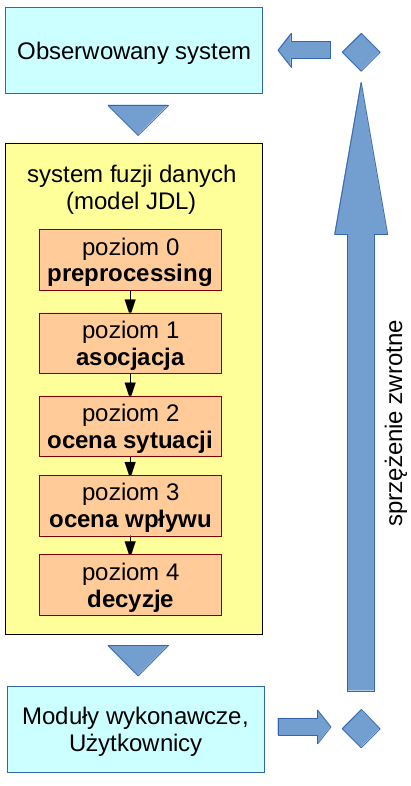
\includegraphics[width=15em,keepaspectratio]{img/jdl}
	\caption{Działanie systemu fuzji danych w modelu JDL}
	\label{jdl}
    \end{center}
\end{figure}

\subsection{System śledzenia}
\par{
Opis modelu JDL stanowi jedynie podstawę dla dalszych rozważań dotyczących konkretnych systemów fuzji danych, pokazuje on jednak generalną logikę stojącą za systemami fuzji niezależnie od metodyki i linii podziału tej logiki na konkretne warstwy.
}
\par{
System śledzenia, dla celów którego tworzony jest opisywany w pracy symulator, jest typowym systemem fuzji informacji. Ma on za zadanie zbierać informacje z wielu czujników rozmieszczonych w środowisku miejskim i na ich podstawie wyznaczać trasy poszczególnych obiektów a także przewidywać dalsze kierunki ich poruszania się.
}
\par{
Z punktu widzenia takiego systemu podstawową informacją dotyczącą obiektów poddawaną fuzji stanowi położenie obiektu, jednakże system ten zakłada możliwość dostarczania przez czujniki większej ilości informacji i może w przyszłości wykorzystywać je by zwiększać swoją skuteczność.
}
\par{
Takie wymagania co do systemu oznaczają, że symulator \textbf{musi} dostarczać do docelowego systemu informace o położeniu obiektów w formie wstępnie przetworzonej. Zakłada się, że obserwacje wykonywane są przez inteligentne czujniki oraz, że czujniki te \textbf{mogą} dostarczać większej ilości informacji.
}
\par{
Ponieważ wyżej zaprezentowany ogólny wstęp dotyczący systemów fuzji danych pozwolił na sformułowanie tego zagadnienia w kontekście pracy, a same systemy fuzji nie są przedmiotem tej pracy, nie będą one bardziej szczegółowo opisywane.
}

\section[Elementy symulowanego środowiska][Elementy symulowanego środowiska]{Elementy symulowanego środowiska}
\par{
Środowiskiem miejskim nazywa się tu ogół obiektów znajdującej się w czterowymiarowej przestrzeni w otoczeniu ludzkich miast, powiązanych wzajemnymi relacjami. Elementami środowiska miejskiego są więc piesi i chodniki, pojazdy i ulice, budynki i ich mieszkańcy, parki wraz z lokalną fauną i florą czy post industrialne ruiny ,,ozdobione'' dzikimi wysypiskami śmieci.
}
\par{
Środowisko miejskie rysuje się więc jako bardzo kompleksowe pojęcie, które nie sposób modelować w całej rozciągłości. Jednakże, z punktu widzenia systemów dozoru, czy też śledzenia, wystarczającym wydaje się być przedstawienie całego środowiska miejskiego jako zbioru obiektów niżej wymienionych typów. Należy pamiętać, że poniżej zaproponowany podział nie jest jedynym możliwym, a został wybrany do omówienia ponieważ pozwalał na jednoczesne zaprezentowanie samego środowiska jak i płynne przejście do jego modelowania w dalszej części pracy.
}
\subsection{Obiekty statyczne}
\par{
Obiektami statycznymi w środowisku miejskim nazywamy wszystkie elementy krajobrazu niezmienne w czasie ale posiadające fizyczną reprezentację, mogącą wchodzić w pośrednią lub bezpośrednią interakcję z innymi obiektami.
}
\par{
W wypadku przestrzeni czterowymiarowej, jaką jest środowisko miejskie, każdy obiekt posiadający fizyczną reprezentację w naturalny sposób opisywany jest bryłą potencjalnie zmienną w czasie. Jako że obiekty statyczne z samej swojej natury są niezmienne w czasie, są one opisywane trójwymiarową bryłą o określonej pozycji w trzech wymiarach i znajdująca się w tej pozycji w każdym punkcie wymiaru czwartego (czasu).
}
\par{
Poza reprezentacją w formie bryły każdy element tego rodzaju może być opisywany w całości lub częściami rozmaitymi parametrami mającymi fizyczny wpływ na inne obiekty z otoczenia jak np.
\begin{itemize}
\item gęstość lub masa,
\item przepuszczalność światła,
\item współczynnik odbicia,
\item współczynnik tarcia;
\end{itemize}
}
\par{
Ilość uwzględnianych właściwości obiektów statycznych zależy od potrzeb tworzonego modelu. Opisywanie poszczególnych własności fizycznych obiektów nie jest przedmiotem tej pracy. Przy tworzeniu ogólnego modelu dla środowiska miejskiego należy jednak uwzględnić fakt, że tego rodzaju właściwości istnieją i w zależności od potrzeb konkretnych badań lista uwzględnianych parametrów może być zmienna.
}
\par{
Przykładami obiektów statycznych są:
\begin{itemize}
\item budynki
\item roślinność
\item znaki drogowe
\item ulice, chodniki
\end{itemize}
}
\subsection{Ścieżki}
\par{
Ulice, chodniki czy inne szlaki po których typowo poruszają się obiekty w środowisku miejskim są określane wspólnym mianem ścieżek. Choć ścieżki same w sobie mają zwykle niezmienną w czasie reprezentacje fizyczną, czyli są obiektami statycznymi, to mają one dodatkowe charakterystyczne znaczenie semantyczne.
}
\par{
Ścieżka wyznacza parametryzowalny szlak, po którym mogą poruszać się obiekty pewnego rodzaju. Wyznaczenie tego rodzaju ścieżek zdaje się być typowe dla obserwatorów rzeczywistego świata stąd też wyróżnienie tego bytu w specjalną grupę.
}
\par{
Wyróżnienie ścieżek ma również praktyczne znaczenie w badaniach --- ścieżki wraz z ich semantyką można bowiem w prosty sposób badać pod względem cech związanych z przepływem i umiejscowieniem na nich obiektów.
}
\subsection{Czujniki}
\par{
Jednym z najistotniejszych elementów opisywanego środowiska jest zdolność obiektów w nim się znajdujących do autonomicznego obserwowania stanu swojego otoczenia. W szczególności wszelkiego rodzaju czujniki stanowiące źródło danych dla docelowego systemu fuzji są w stanie zaobserwować co najmniej część  spośród cech posiadanych przez obiekty w systemie.
}

\subsubsection{Obserwacja środowiska}
\par{
Środowisko miejskie niezależnie od zastosowanego modelu można potraktować jako zbiór informacji (stan) wraz z opisem zasad jego zmian w czasie. Cały stan układu jest maksymalną informacją niesioną przez system. Choć fakt ten wydaje się naturalny, rozpatrując podzbiór informacji dostarczany do poszczególnych czujników warto mieć na względzie, że zawsze będzie on jedynie podzbiorem lub wynikową podzbioru stanu układu.
}

\subsubsection{Stopień przetworzenia danych}
\par{
Rozpatrując charakter czujników należy przede wszystkim skupić się na uwzględnieniu jakie informacje z modelu mogą one uzyskać. Mogą one mieć dwojaki charakter:
\begin{itemize}
\item Bezpośredni --- czujniki odbierają bezpośrednio wielkości znane z modelu środowiska. Tego rodzaju czujniki są zawsze uproszczeniem, ponieważ sam model jest jedynie przybliżeniem rzeczywistości, ale jednocześnie pozwalają na szybkie uzyskanie określonych informacji o określonych cechach systemu, kiedy sam sposób ich pozyskania nie jest przedmiotem badań. Przykładem takiego czujnika może być inteligentna kamera, która dostarcza bezpośrednio odczytów dotyczących pozycji zaobserwowanych obiektów.
\item Fuzyjny --- czujniki odbierają informację jako wynik analizy określonych czujników stanowiący syntezę wielu elementów modelu. Zwykła kamera obserwująca kolejne obrazy będące wypadkową kolejnych stanów modelu jest właśnie takim czujnikiem.
\end{itemize}
W przypadku systemu mającego służyć generowaniu konkretnych informacji, jakim jest opisywany w tej pracy symulator, typowym zdaje się być zastosowanie czujników o charakterze bezpośrednim, co jednakowoż nie przekreśla szansy zastąpienia ich czujnikami fuzyjnym wraz analizatorem ich obserwacji by uzyskać podobne informacje wynikowe w sposób bardziej zbliżony do rzeczywistego.

\subsubsection{Dokładność pomiarów}
\par{
Wszystkie rzeczywiste obserwacje obarczone są pewnym nieredukowalnym błędem \cite{Heisenberg}. Naturalnie wymuszony błąd wynikający z praw fizyki nie jest kluczowy z punktu widzenia realnych obserwacji w makroskali, jednak narzędzia do obserwacji w makroskali są obarczone licznymi błędami wynikającymi z ich konstrukcji, szumów analogowych, losowych zdarzeń, które same w sobie nie muszą być modelowane itp.
}
\par{
Centralne twierdzenie graniczne, mówi, że suma zmiennych o rozkładach charakteryzujących się taką samą wartością oczekiwaną i wariancją upodabnia się do rozkładu normalnego o takich właśnie parametrach. Praktycznym wnioskiem wynikającym z tego twierdzenia, jest fakt, że stosowanie rozkładu normalnego przy sztucznym generowaniu błędów jest statystycznie poprawną metodą zapewniającą dla dużej ilości zaszumionych pomiarów zbliżenie do realnych błędów, które zwykle mają cechy wymagane przez twierdzenie. Wydaje się być to poprawne podejście zarówno w przypadku zastosowania obserwacji bezpośredniej jak i fuzyjnej.
}

\subsection{Obiekty dynamiczne}
\par{
Najważniejszymi z punktu widzenia systemu inwigilacji czy dozoru obiektami są obiekty dynamiczne, ponieważ to właśnie one są przedmiotem bezpośredniej obserwacji.
}
\par{
Obiekty dynamiczne są reaktywnymi elementami wchodzącymi w interakcje z otoczeniem i mogącymi potencjalnie podejmować autonomiczne decyzje dotyczące zmiany własnego stanu. Podobnie jak obiekty statyczne, obiekty dynamiczne mają swoją reprezentację fizyczną w postaci prametryzowalnej bryły.
}
\par{
W środowisku miejskim wyróżnia się dwie najważniejsze grupy obiektów dynamicznych, których przedstawicie są do siebie zbliżeni pod względem pewnych parametrów.
}
\subsubsection{Pojazdy}
\par{
Pojazd w rozumieniu ruchu drogowego definiowany jest jako obiekt fizyczno-psychiczny \cite{TrafficSimulation}. W praktyce bowiem pojazd traktuje się jako tandem pojazd-kierowca (ang. Driver-Vehicle-Element DVE \cite{TrafficSimulation}). Tak jak sam pojazd jest faktycznie odzwierciedleniem fizycznej egzystencji DVE w przestrzeni, tak kierowca odpowiada za jego bieżący stan.
}
\par{ }
\par{
\textbf{Kierowca}
}
\par{
Zadaniem kierowcy w tandemie pojazd-kierowca jest podejmowanie decyzji na podstawie obserwowalnych przez niego właściwości otoczenia. W tym znaczeniu, kierowca jest charakterystycznym rodzajem czujnika, który nie tylko obserwuje pewne własności otocznia ale także podejmuje na ich podstawie decyzje.
}
\par{
Do kierowcy docierają pewne obarczone błędami informacje z zewnątrz (podobnie jak do czujnika), z których na podstawie reguł decyzyjnych wyprowadzane są bieżące akcje polegające na obsłudze interfejsu samochodu (kierownica, pedały, itd.). Stworzenie samych reguł decyzyjnych jest zagadnieniem związanym z tworzeniem sztucznej inteligencji znacznie przewyższającym złożonością zakres tej pracy, i w związku z tym nie będzie tu poruszane. Jednakże, pewne istotne właściwości zachowań ludzkiego kierowcy zostaną tu omówione by wskazać jakie cechy powinny posiadać systemy decyzyjne mające modelować jego działanie.
}
\par{
Podstawowym elementem związanym z reakcjami ludzkimi jest \textbf{czas reakcji}. Czas reakcji składa się z dwóch elementów składowych. Czasu od zdarzenia do rozpoznania konieczności reakcji oraz refleksu czyli czasu jaki upłynie od rozpoznania konieczności reakcji do reakcji mięśniowej \cite{Zatrzymac}.
}
\par{
Pierwszy z tych czasów wynosi statystycznie około $0.7s$ \cite{Zatrzymac}. Drugi natomiast ok. $0.25-0.3s$ \cite{Zatrzymac, ReactionTime} (bardziej precyzyjny rozkład na wykresie \ref{reaction}).
}
\begin{figure}[htb]
    \begin{center}
	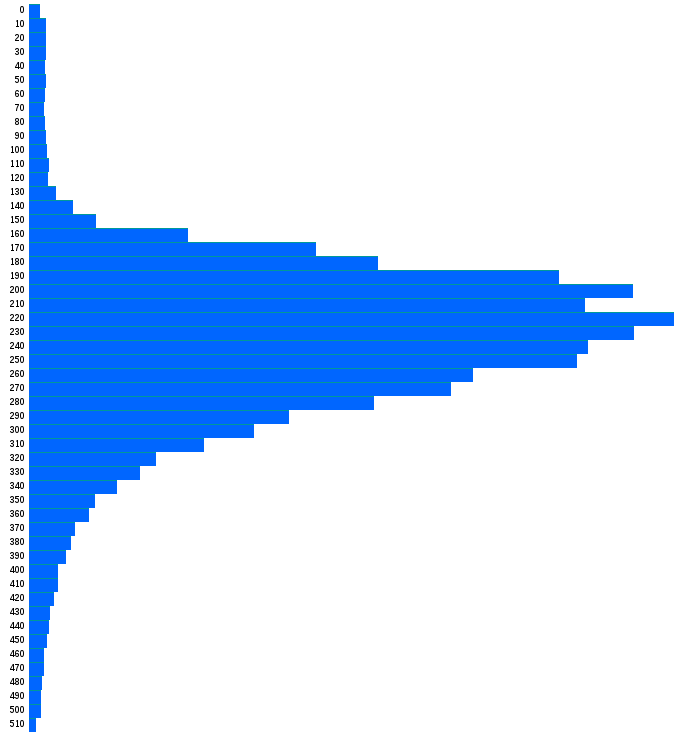
\includegraphics[]{img/reaction_times}
	\caption{Rozkład czasu refleksu (ms) w próbie 6309827 testów zebranych wśród internautów \cite{ReactionTime}}
	\label{reaction}
    \end{center}
\end{figure}

\par{
Sumaryczny czas reakcji wynoszący ok. $1s$ oznacza w przypadku samochodu poruszającego się z prędkością $50km/h$ przejechanie ok. $14m$. Jest to wielkość obserwowalna i istotna w makroskali w związku z tym wydaje się, że w większości wypadków nie należy zaniedbywać czasu reakcji kierowcy przy budowaniu jego modelu.
}
\par{
Innym istotnym aspektem służącym budowie realnego modelu, choć nie koniecznie niezbędnym do statystycznych badań w typowym przypadku są \textbf{błędy kierowcy}, które zdają się być nieuniknione gdy mamy do czynienia z czynnikiem ludzkim. Błędy kierowcy to przede wszystkim:
\begin{itemize}
\renewcommand{\labelitemi}{$\bullet$}
\item Błędna ocena sytuacji --- np. błędna estymacja czasu dojazdu do skrzyżowania.
\item Błędna reakcja --- np. zbyt mocne skręcenie kierownicy.
\item Rozproszenie --- np. niedostrzeżenie zagrożenia.
\item Spowolniona reakcja --- np. w wyniku spożycia alkoholu.
\end{itemize}
}
\par{
Naturalnym elementem szczególnie w kontekście uwzględnienia przez psychikę kierowcy możliwości wystąpienia jego własnych błędów jest \textbf{uwzględnienie poziomu bezpieczeństwa} przez kierującego. Osoba kierująca samochodem uwzględnia ryzyko jakie niesie jazda w określony sposób i nie zakłada swojej idealnej jazdy.
}
\par{
Kolejnym aspektem, na który zwraca uwagę kierowca jest \textbf{ograniczona wiedza} --- często kierowca musi podejmować decyzje nie mając ze względu na pewne ograniczenia (np. widoczności) pełnej wiedzy na temat ruchu w jego okolicy i podejmuje decyzje uwzględniając niejako automatycznie ryzyko związane z wybraniem określonego scenariusza jako domniemanego.
}
\par{
Innym elementem związanym z typową jazdą jest zasada \textbf{ograniczonego zaufania}, która mówi o tym, że nie należy ufać w poprawny czy też bezpieczny sposób reagowania pozostałych uczestników ruchu. Konsekwencją tego, jest np. fakt, że kierowca realnie rusza ze świateł gdy kierowca przed nim zacznie ruszać a nie gdy zobaczy zielone światło. Ma to istotny i nieunikniony wpływ na generalne spowolnienie ruchu.
}
\par{
Kierowca nie decyduje się na jazdę z określoną prędkością biorąc pod uwagę ryzyko jakie niesie za sobą zderzenie i inne wydarzenia na drodze. Kierowcą kierują też względy społeczno-ekonomiczne gdy jedzie zgodnie lub niezgodnie z \textbf{przepisami ruchu drogowego}. Niekiedy tylko konieczność dostosowania prędkości czy innych zachowań do przepisów ruchu zmienia sposób jazdy kierowcy. Co jest szczególnie obserwowalne np. gdy kierowcy reagują zmniejszeniem prędkości na sam widok policyjnego radiowozu.
}
\par{
Powyższe aspekty są jedynie najważniejszymi z punktu widzenia realizmu symulacji i stanowią wierzchołek góry lodowej zagadnienia, psychologicznego dotyczącego elementów składających się na reakcje kierowców.
}
\par{ }
\par{
\textbf{Pojazd}
}
\par{
Zupełnie odrębnym od kierowcy samochodu elementem DVE posiadającym własną specyfikę jest sam pojazd. Pojazd składa się z elementów roboczych, które działają określonymi siłami na otoczenie, oraz z interfejsu, który pozwala regulować działanie elementów roboczych.
}
\par{
Podobnie jak człowiek reaguje z pewnym opóźnieniem, podobnie przeniesienie akcji interfejsu na reakcję elementów roboczych zajmuje pewien czas. Ponieważ jednak czas ten rzędy wielkości niższy od czasu reakcji kierowcy, wydaje być się on pomijalny dla większości zastosowań przy obserwowaniu układu w skali makro.
}
\par{
Pojazdy posiadają pewną charakterystykę przyśpieszenia różną dla różnych ich typów. Przyśpieszenie do $100km/h$ dla nowoczesnego niesportowego samochodu zajmuje ok. $8-12s$, co daje średnie przyśpieszenie ok. $~2.8m/s^2$. Analogiczny zakres dla motocykla to $4-8s$, co daje średnie przyśpieszenie $~4.7m/s^2$. Są to stałe, które można by przyjąć w bardzo uproszczonym modelu zachowując minimalny poziom realizmu. W rzeczywistości należało by się posługiwać charakterystykami przyśpieszenia w zależności od prędkości by ustalać konkretne wartości przyśpieszenia (Rysunek \ref{golf}).
}
\begin{figure}[htb]
    \begin{center}
    	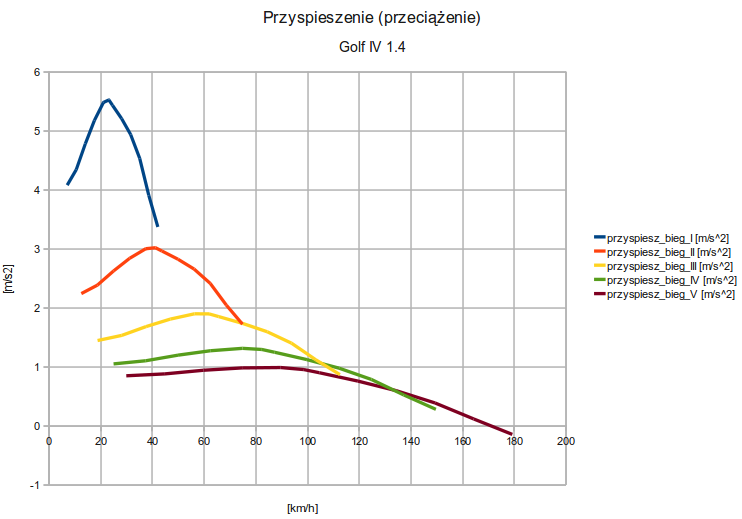
\includegraphics[width=\textwidth,keepaspectratio]{img/golf_acc}
	\caption{Przykład charakterystyki przyśpieszenia od prędkości z uwzględnieniem biegów dla Volksvagena Golf IV 1.4. \cite{Autokult}.}
	\label{golf}
    \end{center}
\end{figure}

\par{
Analogicznie sprawa wygląda jeśli chodzi o opóźnienia (hamowanie), które wg. literatury \cite{Zatrzymac} wynoszą $3.0-4.5m/s^2$ dla samochodów w zależności od rodzaju pojazdu jak i stanu nawierzchni. Oraz $6.0-9.8m/s^2$ dla motocykli.
}
\subsubsection{Piesi}
\par{
Charakterystyka pieszych z punktu widzenia ich zewnętrznej obserwacji jest paradoksalnie bardzo zbliżona do charakterystyki DVE. Można bowiem uznać, że świadomość steruje bezpośrednio interfejsem pojazdu, którym staje się ciało ludzkie --- wtedy wszystkie złożenia dotyczące DVE zostają aktualne.
}
\par{
Naturalnie piesi mają inną fizyczną dynamikę. I tak przeciętna prędkość pieszego wynosi $~5km/h$ \cite{Pedestrians}, a czas średni czas rozpędzania się do tej prędkości wynosi $~2.25s$ \cite{Pedestrians}. Oba te parametry stanowią pewne stałe, które mogą być zastosowane dla uproszczenia, jednak źródła \cite{Pedestrians} podają, iż parametry te zmieniają się w zależności od licznych czynników jak płeć pieszego, dzień tygodnia, rodzaj nawierzchni, pogoda, temperatura, itd. Należy uwzględnić istotne z punktu widzenia celu modelowania korelacje.
}
\chapter{Implementacja symulatora}
\section[Wymagania funkcjonalne][Wymagania funkcjonalne]{Wymagania funkcjonalne}

\par{
Implementowany w ramach tej pracy symulator środowiska miejskiego musi spełniać pewne wymagania, wynikające z możliwości jego późniejszego zastosowania do badań naukowych, a w szczególności do współpracy z systemem fuzji danych obecnie realizowanym przez pana Macieja Grzybka (temat pracy inżynierskiej: \textit{Implementacja algorytmu śledzenia obiektów w systemie fuzji danych} \cite{Grzybek}).
}
\par{
Symulator musi:
\begin{itemize}
	\item Dostarczać dane z czujników rozmieszczonych w mieście w formie wstępnie przetworzonej (na potrzeby fuzji informacji).
	\item Posiadać przynajmniej jeden typ czujnika, który dostarcza przynajmniej informację na temat współrzędnych geograficznych obiektu obserwowanego.
	\item Udostępniać odczyty z czujników przy użyciu uzgodnionego schematu bazy danych dynamicznych.
	\item Odczytywać wejściowe informacje na temat środowiska z określonego schematu bazy danych statycznych (wczytywanie map).
	\item Mieć możliwość dodania implementacji bardziej zaawansowanych rodzajów czujników, a w szczególności posiadających inne właściwości oraz dostarczających innych informacji.
	\item Prezentować symulację w formie graficznej tak, by można było obserwować jej przebieg i konfrontować go z wynikami bieżącego działania systemu fuzji danych.
	\item Umożliwiać regulację natężenia ruchu.
	\item Umożliwiać regulację szybkości symulacji względem czasu rzeczywistego (przyśpieszenie, spowolnienie).
	\item Pozwalać na czasowe wstrzymanie symulacji.
\end{itemize}
}

\section[Metodyka symulacji][Metodyka symulacji]{Metodyka symulacji}
\subsection{Przedmiot symulacji}
\par{
Jak wspomniano w poprzednim rozdziale, dobranie skali integracji symulacji do wybranego zagadnienia jest istotne z punktu widzenia osiągnięcia zamierzonych rezultatów. Wybranie skali zbyt wysokiej ogranicza możliwości zastosowania symulacji i jej rozszerzalność. Wybranie skali zbyt niskiej skutkuje natomiast utrudnieniami implementacyjnymi, wzrostem złożoności obliczeniowej i skomplikowaniem ogólnej zasady działania symulacji, bez rekompensaty w postaci użytecznych możliwości.
}
\par{
Dobranie odpowiedniej skali integracji powinno przede wszystkim uwzględniać skalę w jakiej obserwowany będzie symulowany układ, tak by w tej skali zachowywał się on realistycznie z punktu widzenia celu symulacji. I tak w przypadku przedstawianego w pracy symulatora obserwowane obiekty są obserwowane w stosunkowo wysokiej skali integracji --- jako samochody, piesi i inne elementy makro-świata.
}
\par{
Mając na względzie te potrzeby wydaje się więc, że można traktować te obiekty jako niepodzielne elementy i nie zagłębiać się w ich wewnętrzną specyfikę. Warto jednak uwzględnić fakt, że decyzja ta może uniemożliwiać lub w znacznym stopniu utrudniać niektóre przyszłe rozszerzenia symulacji. I tak, jak nie będzie zapewne stanowiło problemu dodanie do symulacji obsługi zderzeń niesprężystych, gdyż ich obsługa nie wymaga zagłębiania się w budowę obiektów, tak obsługa np. aerodynamiki pojazdów może stanowić znaczące utrudnienie implementacyjne. Należy pamiętać, że nie każde obliczenia mikro skali da się przełożyć na wartości w skali makro.
}
\par{
Licząc się z wyżej wspomnianymi konsekwencjami podjęto decyzję, by elementy świata rozpatrywać w skali abstrakcyjnych obiektów o nieznanej wewnętrznej budowie. Będąc świadomym, iż przedmiotem naszej symulacji są właśnie obiekty makro-świata zawieszone w czterowymiarowej przestrzeni (przestrzeń i czas) i będąc świadomym ich właściwości można przystąpić do dalszego planowania metodyki symulacji.
}

\subsection{Model symulacji}
\par{
Przy założeniu symulacji obiektów makroskopowych należy zadbać o to, by zachowywały się one w sposób realistyczny z punktu widzenia obserwatorów.
}
\par{
Przy rozwiązaniu tego problemu z pomocą przychodzi nam teoria symulacji a także podstawy dynamiki Newtona.
I tak wiemy, że zastosowanie właśnie modelu newtonowskiego do symulowania ruchów obiektów da nam obraz realistyczny z punktu widzenia makro świata.
}
\par{
Podstawowymi wielkościami dynamiki Newtona są siła (\textbf{F}), przyśpieszenie (\textbf{a}) oraz masa (\textit{m}), połączone wzorem:
\begin{center}
$\textbf{F} = m \times \textbf{a}$
\end{center}
Wzór ten opisuje podstawę ruchu i odnosi się właśnie do obiektów makroskopowych o nieznanej lub nieokreślonej strukturze wewnętrznej opisywanych modelami fizycznymi takimi jak punkt materialny lub bryła sztywna.
}
\par{
Dla ciał objętych symulacją również należało znaleźć odpowiedni model fizyczny. Pod uwagę wzięto dwa wyżej wspomniane modele, jako, że zapewniają one realizm symulacji i pozwalają na uwzględnianie licznych czynników zewnętrznych.
}
\par{
Podejście do obiektów symulowanych jak do bryły sztywnej wydaje się być intuicyjne. W naturalny sposób blokuje to możliwość ingerencji w wewnętrzną fizykę ciała, jednocześnie zapewniając wysoki realizm w skali makro.
Takie podejście pozwala na łatwe zasymulowanie wszelkiego rodzaju zdarzeń niesprężystych, także związanych z obrotami, w sposób naturalny ułatwia wykrywanie kolizji i pozwala przewidywać ich przebieg z dużą dokładnością i z zachowaniem wysokiego realizmu.
Niestety model ten ze względu na stopień kompilacji został odrzucony a wybrany został model prostszy --- model punktu materialnego.
\par{
Model punktu materialnego pozwala na wykonywanie wszelkich obliczeń na obiektach, które nie nawiązują między sobą interakcji równie dobrze jak model bryły sztywnej. Jego niewątpliwą wadą jest to, że w razie pojawienia się potrzeby symulowania zderzeń między obiektami pojawił by się spory narzut na dość sztucznej warstwie abstrakcji, która musiała by powstać by obsłużyć zderzenia w sposób realistyczny (dodać do modelu odpowiednie siły, itp.).
Ponadto model ten nie uwzględnia obrotów, ponieważ z jego punktu widzenia obiekty w świecie stają się niematerialnymi punktami bez wymiarów.
Największą i przeważającą zaletą tego modelu była jego prostota, która pozwoliła na szybką implemetację wersji symulatora zdolnej spełniać podstawowe powierzone jej zadania. 
}
\par{
W ramach modelu fizyki punktu materialnego przyjęto, że każdy obiekt w świecie stanowi jeden punkt materialny, który w każdej chwili czasu charakteryzuje się następującymi wartościami:
\begin{itemize}\renewcommand{\labelitemi}{$\bullet$}
\item Siła (wektor trójwymiarowy) z jaką działa ciało na świat stanowiący inercjalny układ odniesienia rozumiany jako statyczny obiekt o nieskończonych wymiarach, względem, którego przemieszczają się ciała (swoista podstawa układu).
\item Masa ciała.
\item Prędkość (wektor trójwymiarowy) z jaką w danej chwili porusza się ciało.
\end{itemize}
Znając te trzy wartości, można określić położenie obiektu w układzie współrzędnych w każdej chwili czasu.
Warto zwrócić uwagę, że tak jak pierwsze dwa z tych parametrów są właściwościami obiektu, tzn. obiekt może je dowolnie zmieniać w czasie, tak prędkość jest wartością wynikającą z dotychczasowej historii danego obiektu i sam obiekt nie jest w stanie wprost zmienić jej wartości (tak jak w rzeczywistości samochód nie może w jednej chwili się zatrzymać, ale może nagle (w modelu przyjęto że nawet w czasie $\Delta t \longrightarrow 0$) zacząć hamować działając z dużą siłą o zwrocie przeciwnym do kierunku jazdy i szybko (ale nie natychmiastowo) wytracić posiadaną prędkość).
}

\subsection{Upływ czasu}
\par{
Ostatnią z punktu widzenia istoty symulacji decyzją jaką należało podjąć było wybranie jednego z dwóch możliwych podejść do symulowania upływu czasu:

\begin{itemize}
\item obliczenia przy założeniu ciągłości czasu,
\item obliczenia przy założeniu czasu skwantowanego (dyskretnego).
\end{itemize}
}
\par{
Pierwsze z podejść jest bliższe realizmowi. Gdyż pomimo, iż w świetle współczesnych badań fizycznych okazuje się, że czas należy rzeczywiście traktować jako parametr zdyskretyzowany, to gęstość jego rzeczywistego ,,próbkowania'' jest tak duża, że nie sposób obsługiwać ją przy użyciu komputera.
Jak wspominano w poprzednim rozdziale, uzyskanie efektu czasu ciągłego sprowadza się do opisania wszystkich elementów symulowanego świata układem równań. W każdej chwili pozycja każdego obiektu może być wyznaczona jako pozycja początkowa przesunięta o wektor wyznaczany z bieżącego równania ruchu danego ciała. Tego rodzaju symulacja zapobiega wszelkiego rodzaju błędom przybliżeń i błędom kwantowania, ma ona jednak inne właściwości, które dyskwalifikują jej użycie.
}
\par{
Warto zwrócić uwagę, że tego typu równania wyznacza się ponownie ilekroć pojawia się jakieś zdarzenie. Przez zdarzenie rozumie się tutaj wszelkie sytuacje mogące wpływać na stan jakiegokolwiek ciała. I tak podstawowymi zdarzeniami w typowym modelu fizycznym są np. zderzenia dwóch ciał. W wypadku symulacji zdarzenie następuje jednak również wtedy, gdy co najmniej jeden z obiektów pod wpływem czynników zewnętrznych zmieni swój stan (tj. siłę lub masę). Niestety wyznaczanie wystąpień tego rodzaju zdarzeń w czasie wydaje się być zadaniem bardzo trudnym. Po pierwsze nie jesteśmy w stanie przewidzieć w jakich sytuacjach obiekt zmienia swój stan --- musimy więc przenieść tę odpowiedzialność na niego, dając mu tym samym wgląd w przyszłość symulacji, co jest niezgodne z logiką procesu. Po drugie obiekt taki musi w swoisty sposób przewidywać przyszłość by zaplanować zdarzenie --- każdy obiekt musi więc mieć pojęcie o całym układzie by być w stanie (i to przy dużym nakładzie obliczeniowym) przewidzieć i zaplanować zdarzenia, które dotyczą jego stanu ruchu.
}
\par{
Rozwiązaniem, które pozwoliło by wdrożyć ideę czasu ciągłego w życie bez konieczności wprowadzania olbrzymiej ilości obliczeń, jest twarde zdefiniowanie w modelu sytuacji w których poszczególne obiekty mogą zmieniać decyzje. Warto jednak zwrócić uwagę, że zmniejsza to decyzyjność pojedynczych jednostek w świecie, co obniża realizm ewentualnie wdrożonej sztucznej inteligencji.
}
\par{
Wyżej wspomniane powody sprawiły, iż zdecydowano się na wybranie wariantu symulacji z czasem jako jednostką skwantowaną. W takiej sytuacji każdy kwant jest punktem decyzji dla każdego obiektu, a przez okres jego trwania ciała poruszają się ze stałymi parametrami (przyśpieszenie, prędkość).
Takie rozwiązanie posiada szereg wad. Po pierwsze, w przypadku potrzeby zasymulowania kolizji pojawia się problem nachodzenia na siebie obiektów. W typowym przypadku zderzenia, w jednym kwancie czasu dwa ciała będą rozłączne a w następnym momencie będą się na siebie nakładały. Jest to niezgodne z modelem fizycznym bryły sztywnej jak i intuicją. Istnieją jednak sposoby radzenia sobie z tego rodzaju problemami --- nie są one jednak przedmiotem tej pracy, a ponieważ w załączonej implementacji zrezygnowano z obsługi zderzeń, nie będą one tutaj rozpatrywane. Warto jednak mieć na względzie ograniczenie samej metodyki symulowania upływu czasu.
}
\par{
Kolejny problem pojawiający się przy obsłudze czasu w kwantach przy zachowaniu szybkości jego upływu w stosunku do czasu rzeczywistego jest fakt, że przy dużym czasie zajmowanym przez każdy krok algorytmu (np. na skutek operacji wejścia wyjścia), wydłuża się czas trwania kwantu czasu. W skrajnych wypadkach może to doprowadzić do kwantów czasu bardzo długich co sprawia, że błąd kwantowania staje się ogromny --- w praktyce może to np. powodować opuszczenie przez obiekty obszaru symulacji.
Problem ten można oczywiście zlikwidować rezygnując z odniesienia czasu symulacji do czasu rzeczywistego (wtedy błąd kwantowania jest stały i z założenia niewielki), jednak jako że takie odniesienie jest jednym z wymagań stawianym symulatorowi, tego typu sytuacje mimo ich nieprecyzyjności należało obsłużyć w sposób możliwe realistyczny z punktu widzenia obserwacji. Zaproponowane rozwiązanie i konkretne miejsca występowania tego problemu opisano w dalszej części pracy.
}
\par{
Dobranie metodyki obsługi upływu czasu stanowi zwieńczenie procesu projektowania działania symulatora. W jego wyniku otrzymano obraz symulatora jako procesu działającego na abstrakcyjnych obiektach makro-świata, obsługiwanych zgodnie z zasadami dynamiki Newtona tak jakby były punktami materialnymi przy jednoczesnym zachowaniu kwantyzacji czasu pozwalającej na swobodne zmiany stanu (rozumianego jako masa i siła) obiektów na skutek ich własnych decyzji w wyznaczonych momentach czasu symulacji.
}

\section[Dobór technologii][Dobór technologii]{Dobór technologii}
\par{
Elementem implementacji aplikacji jest dobranie technologii odpowiadającej wymaganiom stawionym aplikacji. Przez technologie rozumie się w tym wypadku przede wszystkim język programowania oraz system baz danych służący do komunikacji z systemem fuzji danych jak i ten mający odpowiadać za statyczne informacje dotyczące symulowanego środowiska (układ ulic, budynków itp).
Poniższy rozdział traktuje o doborze tych technologii opisując powody ich wyboru.
}
\subsection{Wybór języka programowania}
\subsubsection{Rozszerzalność}
\par{
Symulator według wyżej wyspecyfikowanych wymagań ma na wielu płaszczyznach wspierać możliwości rozszerzania. Obecnie za paradygmat programowania umożliwiający rozszerzenie funkcjonalności w największym stopniu uważa się paradygmat programowania obiektowego.
W związku z tym pod uwagę brane były tylko języki programowania związane z tym paradygmatem, a jednocześnie znane choć w podstawowym stopniu autorowi niniejszej pracy, były to:
\begin{itemize}
\item C++,
\item Java,
\item C\# .
\end{itemize}
}
\subsubsection{Dostępność}
\par{
Istotnym elementem z punktu widzenia każdej aplikacji użytkowej, także tej tworzonej z myślą o prowadzeniu badań naukowych zdaje się być możliwość wykorzystania jej na różnych platformach sprzętowo-systemowych.
}
\par{
I tak spośród wymienionych wcześniej języków programowania tylko dwa pierwsze zdają się pokrywać zakresem swej dostępności porównywalne ilości platform --- są to Java, której kod ze względu na wykorzystanie implementowanej na wiele popularnych platform wirtualnej maszyny może być wykonywany na większości współczesnych urządzeń elektronicznych (nie tylko klasy PC), oraz C++, którego kompilacja i wykonanie ze względu na szeroko dostępne kompilatory dla wielu architektur oraz implementacje biblioteki standardowej nie stanowi problemu dla większości popularnych konfiguracji sprzętowo-systemowych.
}
\par{
Niestety język C\# zdaje się nie być równie dostępny na wielu platformach. Implementacje jego wirtualnej maszyny nie są zbyt szeroko dostępne a nawet jeśli istnieją są generalnie postrzegane jako półśrodek nie do końca spełniający swoją rolę. Z tego względu język C\# został odrzucony i nie będzie rozpatrywany w kolejnych kategoriach doboru.
}
\subsubsection{Wydajność}
\par{
Choć wydajność obliczeń nie jest kluczowym elementem dla aplikacji, czego dowiodły późniejsze badania, to czas obliczeń jest niewątpliwym kosztem i w związku z tym jego minimalizacja zdaje się być istotnym elementem decyzyjnym przy doborze języka programowania.
}
\par{
Język C++ jako język kompilowany bezpośrednio (lub pośrednio) do natywnego kodu maszynowego daje możliwość uzyskania idealnie optymalnego kodu dla danego rozwiązania na danej platformie sprzętowej. W tej kategorii język Java, będący językiem kompilowanym do kodu maszynowego maszyny wirtualnej z natury rzeczy uzyska niższe wyniki wydajnościowe - ze względu niemożliwą do uniknięcia dodatkową warstwę interpretacji w trakcie wykonywania.
}
\par{
Przewaga języka C++ nad Javą jest niezaprzeczalna, jednakże wydajność nie jest głównym kryterium doboru technologii i w związku z tym nie wydaje się by odrzucenie języka Java na tym etapie było rozsądną koncepcją.
}
\subsubsection{Doświadczenie}
\par{
Istotne z punktu widzenia tworzenia aplikacji jest doświadczenie programistyczne w danej technologii. Programista doświadczoniem w danej technologii ma większą szansę na szybkie stworzenie bezawaryjnego i utrzymywalnego oprogramowania.
}
\par{
Doświadczenie autora jest zdecydowanie po stronie języka C++, który jest dla niego naturalnym narzędziem pracy. Język Java znany jest mu tylko pobieżnie i w związku z tym zdaje się on być w tym kontekście mniej rozsądnym wyborem.
}
\subsubsection{Odporność na błędy}
\par{
Naturalną rzeczą związaną nieodłącznie z wytwarzaniem jakiegokolwiek oprogramowania są błędy programistyczne. Języki różnego typu w różny sposób bronią się przed nimi swoją strukturą.
}
\par{
Zarówno język Java jak i język C++ są językami silnie typowanymi. Oznacza to, że za błąd w ich kontekście uważa się zachowania powszechnie uznawane za nielogiczne - stawianie obiektów złych klas w nieokreślonych dla nich kontekstach.
}
\par{
Aspektem typowym dla języka C++, który został wyeliminowany w języku Java jest ręczne zarządzanie pamięcią, które uznawane jest powszechnie za najbardziej błędogenny element tworzenia oprogramowania. W związku z tym, należy zwrócić uwagę, że w tej kwestii język Java, który sam obsługuje zarządzanie pamięcią \cite{Java} nie obciążając tym programisty wydaje się być zauważalnie lepszy. Z drugiej strony w standardzie C++11 wprowadzono do języka C++ sprytne wskaźniki znacząco upraszczające proces zarządzania pamięcią \cite{isoCPP}.
}
\subsubsection{Wybór}
\par{
Mając na względzie powyższe kryteria oceny, wybór wydaje się być nietrywialny. Wydajność obliczeniowa w dzisiejszych czasem nie jest specjalnym kosztem a dla tego konkretnego projektu nie jest kluczowa zwłaszcza jeśli mówimy tylko o zmianach w obrębie tego samego rzędu wielkości. Jednocześnie język chroniący programistę przed jego własnymi błędami zdaje się mieć tu zauważalną przewagę. W praktyce jednak najbardziej kluczowe zdaje się być doświadczenie programistyczne autora tej pracy, które zaważyło o wyborze języka C++.
}

\subsection{Wybór silnika bazy danych}
\par{
Pod uwagę brano następujące silniki baz danych:
\begin{itemize}
\item ORACLE DB --- został odrzucony ze względu na komercyjny charakter, który z przyczyn ideologicznych wydaje się nieodpowiednią bazą dla mogących mieć coraz bardziej rozległy charakter badań naukowych.
\item PostgreSQL --- posiadający zaawansowane funkcje i zbudowany poprawnie przyzwoity RDBMS --- stale rozwijający się i darmowy projekt o otwartym kodzie źródłowym.
\item MySQL --- przejęta przez firmę ORACLE alternatywa dla PostgreSQL. Ze względu na wspomniane przejęcie praw do bazy przez firmę ORACLE została odrzucona ponieważ nie do końca znana jest jeszcze polityka firmy względem tej bazy.
\item sqLite --- RDBMS będący w zasadzie bibliotką języka C++ --- nie wymaga dodatkowego serwera. Jego wadą jest znacząca mniejsza wydajność. W przypadku tego projektu wydajność bazy zdaje się być kluczowym elementem (co potwierdziły późniejsze badania) w związku z czym baza ta została odrzucona.
\end{itemize}
Mając powyższe na względzie wybór RDBMSa padł na PostreSQL.
}

\subsection{Wybór technologii tworzenia interfejsu}
\par{
Wybór technologii interfejsu nie był kluczowy dla projektu, dlatego autor wybrał w zasadzie jedyną dobrze znaną sobie bibliotekę umożliwiającą tworzenie przenośnych interfejsów graficznych --- bibliotekę Qt \cite{Qt}. Biblioteka zdawała się być wystarczająco dobrym rozwiązaniem w związku z czym poszukiwanie alternatywnych rozwiązań wydawało się bezzasadne, zwłaszcza że prezentowanie wyników symulacji nie jest kluczowe z punktu widzenia celu pracy.
}

\section[Projekt bazy danych][Projekt bazy danych]{Projekt bazy danych}
\par{
W ramach symulatora wykorzystywane są dwie odrębne bazy danych. Jedna (baza danych dynamicznych) stanowi główne wyjście aplikacji i służy do zapisu odczytów z czujników umieszczonych wewnątrz symulacji. Druga z baz --- baza statyczna --- służy do opisywania środowiska miejskiego, a w zasadzie jego statycznych elementów.
}

\subsection{Baza danych statycznych}
\par{
Zadaniem bazy danych statycznych jest przechowywanie układu ulic i obiektów statycznych w symulowanym środowisku miejskim. Symulator w pierwszej fazie swojego działania (inicjalizacji) będzie wczytywał tego rodzaju dane by pracować na nich przez cały czas symulacji.
}
\par{
Kwestią dyskusyjną było umieszczenie w bazie danych statycznych umiejscowienia czujników, ponieważ mają one charakter odpowiadający jej specyfice (są niezmienne przez cały czas symulacji). Jednakże, ze względu na to, że do danych tych odnosi się baza dynamiczna, by uniknąć niepotrzebnej zależności jednej bazy od drugiej zdecydowano by umiejscowienie czujników przenieść do bazy danych dynamicznych.
}
\par{
Baza danych statycznych zawiera więc:
\begin{itemize}
\item układ ulic --- rozumiany jako graf geometryczny
\item umiejscowienie i kształt budynków --- traktowanych jako graniastosłupy
\end{itemize}
Szczegóły bazy można zobaczyć na diagramie ER przedstawionym na rysunku \ref{static_db}.
}
\begin{figure}[htb]
    \begin{center}
	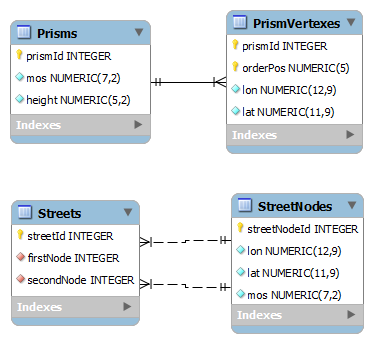
\includegraphics[width=25em]{img/static_db}
	\caption{Diagram ER bazy danych statycznych.}
	\label{static_db}
    \end{center}
\end{figure}

\subsection{Baza danych dynamicznych}
\par{
Baza danych dynamicznych ma za zadanie zbierać informacje z czujników i stanowić element komunikujący symulator z dalszymi systemami bazującymi na jego wyjściu. Struktura tej bazy musi być w związku z tym możliwie elastyczna --- by nie ograniczać przyszłego rozwoju całego ciągu narzędzi. Struktura ta została zaprojektowana we współpracy z twórcą oprogramowania korzystającego z wyników symulatora.
}
\par{
Diagram ER bazy danych dynamicznych przedstawiono na rysunku \ref{dynamic_db}.
}
\begin{figure}[htb]
    \begin{center}
	\includegraphics[width=\textwidth,keepaspectratio]{img/dynamic_db}
	\caption{Diagram ER bazy danych dynamicznych.}
	\label{dynamic_db}
    \end{center}
\end{figure}

\subsubsection{Raport wykrycia}
\par{
Podstawowym pojęciem w przypadku bazy danych dynamicznych to \textit{raport o zauważeniu obiektu} (\textit{Detection Report}). Raport taki, zawiera w minimalnym przypadku współrzędne dokonanej obserwacji oraz jej czas. Jednakże, należy zwrócić uwagę, że ogólny projekt symulatora i całego ciągu narzędziowego dopuszcza możliwość dodawania do takiego raportu dodatkowych informacji w związku z czym baza musi posiadać dynamiczną strukturę, która umożliwia zapisanie tego rodzaju danych.
}
\par{
Zaproponowana struktura pozwala na łączenie każdego raportu wykrycia z dowolną ilością \textit{wartości dodatkowych} (\textit{Feature Value}). Wartość dodatkowa  zapisywana jest w postaci ciągu znaków którego interpretacja zależy od aplikacji, która dodatkowo może posiłkować się informacjami dotyczącymi typu danej --- możliwej do uzyskania z opisu konkretnej wartości dodatkowej.
}
\par{
Każda wartość dodatkowa odnosi się bowiem do \textit{definicji wartości dodatkowej} (\textit{Feature for Sensor}). Tabela ta opisuje każdą klasę wartości dodatkowych typem informacji jaką za sobą ta klasa niesie oraz jej nazwą. Interpretacja znaczenia typu, który jest opisywany ciągiem znaków zależy od narzędzia docelowego, zakłada się jednak, że w typowym wypadku ciągi znaków będą zawierały nazwy typów zgodne z odpowiadającymi im typami w języku C++.
}
\subsubsection{Czujnik}
\par{
Innym elementem, który musi być opisany przez dynamiczną bazę danych, by uniknąć niepotrzebnej zależności od bazy danych statycznych jest czujnik. Każdy raport o zauważeniu obiektu musi posiadać informację na temat czujnika, z którego pochodzi. Podstawową informacją dotyczącą każdego czujnika jest jego położenie w przestrzeni oraz maksymalny zasięg. Maksymalny zasięg to odległość z jakiej dany czujnik może przy idealnych warunkach zebrać jakiekolwiek informacje.
}
\par{
Poza podstawowymi informacjami każdy czujnik może mieć swoją charakterystykę opisującą jego działanie (np. pole widzenia wyrażone w stopniach). Ponieważ typowo czujniki tego samego typu charakteryzują się podobnymi atrybutami, wprowadzono pojęcie typu opisywanego opcjonalnie nazwą. Każdy typ posiada zestaw atrybutów charakterystycznych dla siebie. Każdy atrybut posiada typ i opcjonalnie nazwę. Wiele czujników może wymagać takich samych informacji.
}
\par{
Dokładną strukturę bazy dynamicznej przedstawia poniższy diagram ER.
}


\section[Architektura systemu][Architektura systemu]{Architektura systemu}
\par{
Zastosowanie poprawnej struktury architektonicznej całej aplikacji zdaje się mieć kluczowe znaczenie dla możliwości jej rozwoju, utrzymania jak i bezbłędnego napisania. Poprawna architektura chroni bowiem programistę przed jego własnymi błędami lub też pozwala na ich łatwe odnajdowanie.
}
\subsection{Model MVC}
\subsubsection{O modelu}
\par{
Model MVC (Model-View-Controller, z ang. Model-Widok-Kontroler) został zaproponowany jako całość w 1979 przez Trygve Reenskaug \cite{MVC}, choć --- co jest typowe dla wzorców projektowych --- był on wykorzystywany wcześniej niż został opisany. 
}
\par{
Model MVC dzieli aplikację lub jej część na trzy warstwy:
\begin{itemize}
\item \textbf{Model} --- w założeniu stanowi element odpowiadający za przechowywanie i obróbkę danych na jakich pracuje dane oprogramowanie. Model posiada interfejs umożliwiający wykonywanie akcji na danych oraz dostęp do nich. Może, choć nie musi wykonywać akacje na danych niezależnie od wywołań z zewnątrz.
\item \textbf{Kontroler} --- jego zadaniem jest przechowywanie kontekstu aplikacji, oraz przekazywanie zadań sterowania z widoku do modelu a także pobieranie z modelu informacji, których zażąda widok.
\item \textbf{Widok} --- odpowiada za prezentację danych użytkownikowi. Nie ma on świadomości procesów zachodzących na danych, zna jedynie sposób ich prezentacji oraz akcje jakie można na nich wykonać. Nie jest jednak świadom jak owe akcje wpłyną na te dane.
\end{itemize}
}
\par{
Podział taki zapewnia separację danych od sposobu ich prezentacji, co pozwala zbudować aplikacje o jednej funkcjonalności na wiele różnych sposobów z wieloma różnymi interfejsami utrzymując tylko jeden moduł odpowiedzialny za logikę aplikacji (model).
}
\subsubsection{Zastosowanie w aplikacji}
\par{
Model MVC zdawał się idealnie pasować do prezentowanego w pracy symulatora --- posiada on bowiem całą funkcjonalność symulacji oraz zapisu danych, która jest całkowicie niezależna od sposobu prezentowania danych użytkownikowi. Brak jawnej separacji między modelem a interfejsem użytkownika zapewne doprowadził by do wymieszania tych warstw co mogło by spowodować między innymi następujące problemy:
\begin{itemize}
\renewcommand{\labelitemi}{$\bullet$}
\item Utworzenie zależności symulacji od działania intefrejsu --- co prowadzi do braku możliwości prostej zamiany interfejsu w przyszłości.
\item Rozsynchronizowanie stanu modelu z widokiem.
\item Nieczytelność kodu spowodowana przeplataniem się kodu odpowiedzialnego za wyświetlanie danych i ich obsługę.
\end{itemize}
}
\subsection{Wielowątkowość}
\par{
Opisywany symulator został zaprojektowany by funkcjonować z wykorzystaniem trzech wątków:
\begin{enumerate}
\item Odpowiedzialnego za obsługę modelu --- uruchamianego na początku symulacji i zmieniającego model wraz z upływem czasu.
\item Odpowiedzialnego za widok --- wątek główny przekazany jest we władanie biblioteki Qt, która uruchamia własną kolejkę komunikatów i w jej ramach obsługuje interfejs użytkownika.
\item Odpowiedzialnego za kontroler --- odpowiada on za przekazywanie informacji między widokiem a modelem.
\end{enumerate}
}
\subsubsection{Biblioteka boost::thread}
\par{
Do uruchamiania wątków wykorzystano przenośną bibliotkę boost::thread \cite{Boost} umożliwiającą zaawansowane zarządzanie i synchronizację wątków. Biblioteka ta pozwoliła na łatwe uruchomienie wątków i zsynchronizowanie ich zakończenia. Pozwala ona bowiem na uruchomienie nowego wątku w oparciu o zadany obiekt-funktor \cite{Boost} oraz zawieszenie dowolnego wątku posiadającego referencję do wątku na zawieszenie się w oczekiwaniu na jego zakończenie (join) \cite{Boost}. Te funkcjonalności były wystarczające dla zastosowań projektu.
}
\par{
Biblioteka boost::thread została wybrana ponieważ jest dostępna dla wielu platform oraz nie wprowadza dodatkowych zależności (z tego powodu nie wybrano wątków dostarczanych przez bibliotekę Qt).
}

\subsubsection{Problemy synchronizacji}
\par{
Za każdym razem gdy aplikacja pracuje z wykorzystaniem więcej niż jednego wątku a między wątkami istnieje jakakolwiek forma komunikacji mamy do czynienia z problemami synchronizacji.
}
\par{
W przypadku opisywanego symulatora rozwiązaniem wszystkich problemów zdaje się być zwężenie wszelkiej komunikacji między-wątkowej do bezpiecznych wątkowo  kolejek komunikatów pozwalających na zawieszenie wątku w oczekiwaniu na pojawienie się wiadomości. Dzięki ich zastosowaniu każdy wątek odbiera wiadomości w dogodnym dla siebie momencie i sam zmienia swoje dane --- jego dane zmieniane są tylko przez jeden wątek więc nie ma możliwości ich rozsynchronizowania.
\par{
Wadą takiego rozwiązania zdaje się być zwiększona złożoności kodu ponieważ zamiast prostych wołań metod mamy do czynienia z dodawaniem wiadomości do kolejek. Z drugiej jednak strony, dzięki temu wyraźnie widać w kodzie miejsca, gdzie następuje komunikacja między kluczowymi modułami aplikacji, co ułatwia jego zrozumienie.
}


\section[Architektura modelu][Architektura modelu]{Architektura modelu}
\par{
Zaprojektowanie właściwej architektury modelu jest kluczowe dla celu tej pracy. Poprawnie zaprojektowany model powinien być możliwie elastyczny, a jednocześnie pozwalać na szybkie zaimplementowanie minimalnego podzbioru funkcjonalności pozwalającego na uruchomienie symulacji.
}
\par{
Kompletny diagram klas modelu przedstawiono na rysunku \ref{model_cd}.
}
\begin{figure}[htb]
    \begin{center}
	\includegraphics[width=\textwidth,keepaspectratio]{img/model_cd}
	\caption{Kompletny diagram klas modelu.}
	\label{model_cd}
    \end{center}
\end{figure}

\subsection{Obiekty świata}
\par{
Podstawowym elementem symulowanego środowiska jest \textit{świat}, będący obiektem obsługującym zasady fizyki opisane w wyżej wspomnianym modelu. \textit{Obiekt świata} nie wpływa jednak bezpośrednio na stan obiektów, które tym zasadom podlegają.
}
\par{
Obiekty wewnątrz modelu dzielą się na trzy grupy:
\begin{enumerate}
\item Obiekty posiadające reprezentację fizyczną, np. budynki
\item Obiekty odbierające informacje o otoczeniu, np. czujniki
\item Obiekty posiadający obie powyższe właściwości, np. pojazdy
\end{enumerate}
Z tego rodzaju podziału wynika możliwość wyodrębnienia klasy obserwator (\textit{Observer}), klasy reprezentującej obiekty posiadające reprezentacje fizyczną (\textit{Object}) oraz klasy posiadającej reprezetnację fizyczną i możliwość odbierania informacji o otoczeniu (\textit{LiveObject}). Podział ten przedawia rysunek \ref{obj_obs_cd}.
}
\begin{figure}[htb]
    \begin{center}
	\includegraphics[width=30em]{img/obj_obs_cd}
	\caption{Podział obiektów na obserwatorów i fizyczne obiekty.}
	\label{obj_obs_cd}
    \end{center}
\end{figure}

\par{
Do zadań \textit{obserwatorów} należy obsługa reakcji na zdarzenia nadchodzące z zewnątrz. Klasa \textit{Object} natomiast ma za zadanie udostępniać wielkości fizyczne jakimi manipuluje autonomicznie obiekt --- siłę i masę.
}
\par{
Tylko obserwator jest świadom upływu czasu symulacji --- może on zmieniać swój stan wraz z jego upływem. Obiekt nie posiada takiej możliwości --- obsługa zmian jego stanu musi się odbywać przez interfejs obserwatora. W ten sposób obiekty statyczne nie będące obserwatorami automatycznie nie mogą zmieniać swojego stanu w czasie.
}
\par{
Obserwator otrzymuje wszelkie informacje w formie \textit{zrzutów} z obiektów fizycznych (czyli podzbioru informacji posiadanych na temat obiektów klasy \textit{Object} przez \textit{obiekt świata}). Zrzut zawiera nie więcej informacji niż posiada na temat obiektu \textit{świat} (ponieważ jest przezeń tworzony), ale może zawierać ich mniej --- \textit{świat} dobiera informacje przeznaczone dla poszczególnych obserwatorów.
}

\subsubsection{Wzorzec wizytatora}
\par{
Z punktu widzenia implementacji istotnym zdaje się być sposób zapewnienia obserwatorom możliwości obsługi poszczególnych rodzajów (typów) \textit{zrzutów} z obiektów. Każdy z typów może być przecież traktowany osobno, a sam typ jest już dla obserwatora rozpoznawalną informacją --- jeśli świat nie chciał by takiej informacji dostarczać, nie tworzył by danego podtypu zrzutu.
}
\par{
Z pomocą w tej sytuacji przychodzi wzorzec wizytatora pozwalający obiektowi wchodzić w interakcje z obiektami z określonej hierarchii dziedziczenia w taki sposób by musiał on zapewnić specyficzną obsługę dla każdego jej podtypu.
}
\par{
W tym konkretnym zastosowaniu \textit{obserwatorzy} wizytują \textit{zrzuty} i w ten sposób mogą ustawiać swój wewnętrzny stan i podejmować konkretne decyzje. W zależności od potrzeb \textit{obserwator} może albo reagować na kolejne wizytowane \textit{zrzuty} lub podczas wizytacji zbierać informacje by podjąć decyzję po przejrzeniu wszystkich dostarczonych do niego danych.
}

\subsection{Upływ czasu}
\par{
W przypadku implementacji symulatora z modelem dynamicznym kluczowe jest poprawne i spójne obsłużenie upływu czasu dla modelu. W przypadku tej implementacji zastosowano powszechnie stosowaną w systemach czasu rzeczywistego architekturę żywej pętli. Architektura ta zapewnia możliwe wysoką precyzję przy odliczaniu czasu, jej niewątpliwą wadą jest natomiast nieoptymalne wykorzystanie zasobów.
}
\subsubsection{Biblioteka boost::chrono}
\par{
Inną od samej architektury kwestią jest zapewnienie spójnego systemu przeliczania czasu, szczególnie w kontekście czasu względnego względem realnego. Z pomocą przychodzi biblioteka boost::chrono \cite{Boost} z zestawu bibliotek boost.
\par{
W chwili bieżącej biblioteka chrono jest elementem biblioteki standardowej języka C++, jednak w momencie rozpoczynania pracy nad aplikacją nie była ona jeszcze zbyt szeroko zaimplementowana w związku z tym zdecydowano się na jej pierwowzór - boost::chrono.
}
\par{
Biblioteka ta pozwala na wykonywanie wszelkich operacji związanych z czasem z uwzględnieniem spójności typów. Biblioteka rozróżnia moment w czasie, zakres czasów czy różnice w czasie jako odrębne typy i pozwala wykonywać na nich tylko takie operacje, które mają logiczny sens --- za każdym razem zwracając odpowiednio uzasadniony nowy typ.
}
\subsubsection{Wzorzec obserwatora}
\par{
Odrębną sprawą od samego przeliczania czasu jest fakt, że wiele obiektów w systemie powinno być w stanie reagować na upływ czasu w symulacji. Stworzono do tego celu interfejs \textit{SimulationPart}, dzięki czemu każdy element symulacji jest informowany gdy w symulacja posuwa się o kolejny krok.
}
\par{
Zastosowano to wzorzec obserwatora, gdzie wszystkie elementy symulacji (w tym w szczególności \textit{obserwatorzy}, którzy są elementami symulacji) obserwują \textit{symulację}. \textit{Symulacja} powiadamia ich gdy upływa pewien czas.
}

\subsection{Połączenie z bazą danych}
\par{
Istotnym elementem modelu symulatora jest komunikacja z bazą danych --- jest ona kluczowa zarówno dla inicjalizacji modelu jak i dla przekazywania jego wyjścia.
}
\subsubsection{Biblioteka pqxx}
\par{
Ponieważ jako silnik bazy danych wybrano \textit{PostgreSQL} należało odnaleźć możliwie obiektową bibliotekę z interfejsem w języku C++ pozwalającą na komuniakcję z taką bazą. Typowym rozwiązaniem jest zastosowanie biblioteki \textit{pqxx} \cite{pqxx}.
}
\par{
Biblioteka \textit{pqxx} zapewnia spójny interfejs pozwalający na pełny dostęp do bazy \textit{PostgreSQL} na poziomie klienckim (tj. przy użyciu zapytań). Jest to funkcjonalność oczekiwana przez bibliotekę mającą zapewniać komunikację z bazą w symulatorze.
}
\subsubsection{ORM}
\par{
ORM (ang. \textit{Object-Relational Mapping}, \textit{Mapowanie Obiektowo-Relacyjne}), to proces zamiany danych relacyjnych na dane obiektowe --- typowy gdy chcemy wykorzystać relacyjną bazę danych do przechowywania danych na potrzeby aplikacji obiektowych.
}
\par{
Najprostsza zamiana krotek na obiekty polega na stworzeniu obiektów o strukturze identycznej ze strukturą krotki i przepisaniu w odpowiednie atrybuty obiektu wartości pobranych z krotki. Również relacje typowo przekładalne są na wskaźniki lub referencje do odpowiednich obiektów klas powiązanych relacjami w bazie relacyjnej.
}
\par{
W przypadku opisywanej aplikacji takie mapowanie zdawało się być wystarczające, w związku z czym zbudowano bibliotekę pozwalającą na uzyskiwanie danych z RDBMS przy użyciu metod wykonujących odpowiednie zapytania, a zwracających gotowe do dalszej pracy obiekty oczekiwane w pozostałych częściach aplikacji.
}

\subsection{Zarządzanie elementami symulacji}
\par{
Istotnym elementem symulacji jest tworzenie i usuwanie nowych obiektów --- elementów tejże symulacji. Do tego celu powołano klasę będącą podklasą elementu symulacji, mającą dostęp do wszystkich danych \textit{świata} - który decyduje arbitralnie  wg. znanych sobie reguł o tworzeniu lub usuwaniu obiektów.
}
\par{
W przypadku przykładowej implementacji zarządca obiektów dodaje obiekty (lub usuwa je) losowo gdy ich ilość w świecie jest różna od zadanej. Implementacja ta jest możliwie prosta --- ponieważ pozwalała ona na szybkie uzyskanie działającej symulacji a dodanie do zarządcy większej logiki wymaga jedynie opisania właśnie tej logiki --- architektura pozwala na jego swobodną rozbudowę.
}

\subsection{Obsługa fizyki}
\par{
\textit{Świat} jest klasą, która odpowiada za przekładnie akcji elementów symulacji na ich stan w symulowanym świecie. \textit{Świat} odbiera informacje o sile i masie od obiektów i na ich podstawie wyznacza ich przyśpieszenie, a w konsekwencji chwilową prędkość.
}
\par{
Zadaniem \textit{świata} jest również obsługa mapy, jako że może ona wpływać na reakcje elementów symulacji.
}

\subsection{Komunikacja ze światem (API)}
\par{
Zadaniem głównej klasy modelu jest obsługa komunikacji z kontrolerem. W implementacji realizowanej w ramach tej pracy, model udostępnia zewnętrznym modułom następujące operacje:
\begin{itemize}
\item wystartuj symulację,
\item wstrzymaj symulację,
\item zatrzymaj symulację,
\item pobierz bieżący stan symulacji (zrzut),
\item pobierz bieżący stan mapy (zrzut),
\item pobierz bieżącą szybkość symulacji,
\item zmień szybkość symulacji na zadaną,
\item zarejestruj obserwatora stanu,
\item wyrejestruj obserwatora stanu.
\end{itemize}
}
\subsubsection{Obserwacja stanu symulacji}
\par{
Zewnętrzne moduły mogą rejestrować się wewnątrz modelu jako obserwatorzy (w rozumieniu wzorca obserwatora) by być informowanymi o zmianach w modelu. Obserwator jest informowany za każdym razem, gdy model zmienia swój stan i tworzy nowe zrzuty mapy bądź obiektów w świecie. W typowym wypadku reakcją na taką notyfikację jest pobranie nowego stanu i jego wykorzystanie do swoich celów przez obserwatora.
}

\section[Architektura widoku][Architektura widoku]{Architektura widoku}
\par{
Zadaniem widoku jest prezentowanie bieżącego stanu symulacji jak i udostępnienie odpowiednich kontrolek pozwalających sterować modelem.
}
\par{
Realizacja takiego zadania wymaga od biblioteki dwojakich możliwości --- po pierwsze prezentacji w formie graficznej układu brył, czyli udostępnienie sceny dla wizualizacji 3D lub płótna dla wizualizacji 2D. Po drugie udostępnienia interaktywnych kontrolek pozwalających na wysyłanie do modelu określonych rozkazów. Biblioteka Qt zdaje się odpowiadać na obydwa te wymagania.
}
\subsection{Biblioteka Qt}
\par{
Podstawowym elementem biblioteki \textit{Qt} jest zapewnienie synchronicznej i asynchronicznej komunikacji między wątkami jak i w ich obrębie za pomocą kolejki komunikatów obsługiwanej poza świadomością użytkownika.
}
\par{
Biblioteka ta, udostępnia mechanizm sygnałów i slotów jako interfejs pozwalający na łatwe korzystanie wyżej wspomnianego mechanizmu. Niestety ponieważ składniowo opis tego mechanizmu jest szerszy niż składnia języka C++, do jego tłumaczenia wykorzystywane jest dodatkowe narzędzie --- MOC (\textit{Meta-Object Compiler}).
}
\par{
Mechanizm ten pozwala jednak na szybkie definiowanie luźnych wiązań w obrębie modułów kontrolowanych przez bibliotekę \textit{Qt} --- co jest niewątpliwie użyteczną cechą w przypadku interfejsów graficznych.
}
\subsubsection{QtGui}
\par{
Biblioteka \textit{QtGui} pozwala na tworzenie interaktywnych formularzy z wykorzystaniem odpowiednich dla danej platformy metod --- typowo z wykorzystaniem natywnych kontrolek platformy. Głównym zadaniem tej biblioteki zdaje się być odcięcie logiki działania interfejsów graficznych od ich konkretnej implementacji. Dlatego ten sam kod wykorzystujący bibliotekę \textit{Qt} skompilowany na różnych platformach daje inny kod wynikowy ale jednocześnie podobne odczucia użytkownika odnośnie interfejsu.
}
\subsubsection{QGraphicsLibrary}
\par{
\textit{QGraphicsLibary} to biblioteka pozwalająca między innymi na definiowane 2 wymiarowych scen i wykonywanie na nich akcji logicznych a jednocześnie na bezpośrednie prezentowanie ich na ekranie w obrębie kontrolek biblioteki \textit{QtGui}. Funkcjonalność ta zdawała się idealnie odpowiadać potrzebom wizualizacyjnym prezentowanej aplikacji i w związku z tym została ona wykorzystana do prezentowania użytkownikowi bieżącego stanu aplikacji.
}
\par{
Ponieważ widok jest obserwatorem stanu modelu, otrzymuje on informacje o jego nowym stanie i żąda nowych zrzutów kiedy uzna to za konieczne. Zrzut zawiera informacje na temat położenia, typu oraz innych atrybutów obiektu. W związku z tym, stosując ponownie wzorzec wizytora odpowiedni komponent widoku jest w stanie zmienić tę reprezentacje na odpowiadającą jej reprezentacje graficzną. Pozwala to na zachowanie kluczowej z punktu widzenia architektury aplikacji separacji między warstwami -- model nie ma żadnej informacji na temat sposobu prezentowania swojego stanu.
}

\section[Architektura kontrolera][Architektura kontrolera]{Architektura kontrolera}
\par{ 
Ostatnią warstwą modelu MVC, jest kontroler. Jego zadanie to przede wszystkim przekładanie zapytań widoku na operacje modelu oraz utrzymywanie stanu aplikacji.
}
\par{
Ponieważ zdecydowano się na rozdzielenie modelu z biblioteką \textit{Qt} by nie wprowadzać trudnej do usunięcia zależności, mechanizm sygnałów i slotów, musiał zostać zamieniony na typowe dla języka C++ wołania metod.
}
\par{
Dodatkowym argumentem, który sugerował by tak postąpić był fakt, że praktyka pokazuje, że zastosowanie mechanizmów sygnałów i slotów, ze względu na brak jakichkolwiek ograniczeń w kwestii dodawania zdarzeń z dowolnego miejsca aplikacji, powoduje, że aplikacja przestaje bronić się przed próbami niezgodnego z architekturą przepływu informacji. Ponadto sygnały i sloty nie mają mechanizmów wykrywania błędów w czasie kompilacji --- weryfikacja ich działania odbywa się dopiero w czasie działania aplikacji.
}
\par{
Odcięcie od mechanizmów \textit{Qt} wykonano z wykorzystaniem prostego mechanizmu przekładania zdarzeń \textit{Qt} na wiadomości pojawiającej się w kolejce komunikatów. Obsługa każdego ze slotów tworzy na podstawie otrzymanych parametrów odpowiedni typ wiadomości i umieszcza tę wiadomość w kolejce komunikatów. Wątek kontrolera będący już niezależnym od biblioteki Qt wyjmuje kolejne wiadomości z tej kolejki i zapewnia im odpowiednią obsługę.
}
\chapter{Badanie wydajności}
\par{ Treść... }


\appendix

% tutaj załączniki

%\chapter*{Bibliografia}
\nocite{*}
\bibliographystyle{plplain}
%\bibliographystylebk{plplain}
%\bibliographystylest{plplain}
%\bibliographystyledoc{plplain}
% \bibliographystyleweb{plplain}
%\bibliographybk{BIB/books}
%\bibliographyst{BIB/books}
%\bibliographydoc{BIB/books}
% \bibliographyweb{BIB/books}

% \bibliography{bib/verificard,bib/jml,bib/daikon}
\bibliography{bib/daikon,bib/statistics,bib/other}

\end{document}

% ex: set tabstop=4 shiftwidth=4 softtabstop=4 noexpandtab fileformat=unix filetype=tex spelllang=pl,en spell:


